\chapter{Úvod}
\label{uvod}

V dávných dobách byla hudba pouze monofonní, což znamená, 
že se skládala ze samostatných melodií bez doprovodu.
Až v průběhu středověku byla vynalezena harmonie.
Tím rozumíme skupinu tónů, které zní všechny ve stejnou dobu.
Použitím harmonie získáme bohatší a barevnější hudbu.
Rozšiřování melodií o akordy, souzvuky, je umělecký proces,
a po muzikantovi či skladateli vyžaduje znalost přechodů akordů a harmonie tónů.
Nabytí těchto znalostí je jedna věc, 
avšak jejich uvedení do praxe může být pro laika 
nebo hudebníka bez dostatečných zkušeností velmi obtížné.
\par

Tématem této práce je vytvořit nástroj, 
který k známé melodii doplní vhodný harmonický doprovod.
Tento nástroj pak může být užitečný právě pro hudební začátečníky,
kteří si nejsou svými schopnostmi jistí. 
Dále může být využit v procesu skládání plnohodnotné hudby počítačem.
V takovém případě by navrhovaný systém následoval za generátorem melodie
a jeho výsledek doplňoval.
Skládání hudby, tedy i harmonie, je umění a vyžaduje hudební cit,
proto podobné systémy bývají zatíženy určitou chybou, 
popřípadě může být jejich výtvor poněkud nudný oproti profesionálnímu složení.
\par

Cílem práce je seznámit se s problematikou automatické harmonizace na základě znalosti melodie,
s principem a využitím strojového učení v této úloze, a to zejména s neuronovými sítěmi.
Dalším bodem je navržení systému, který automatické generování harmonie umožní.
Poté implementovat daný systém s pomocí vhodného frameworku pro neuronové sítě.
Implementovaný systém je potřeba otestovat na vhodné datové sadě. 
Ta bude obsahovat přepis rozličných písniček ze serveru \url{www.hooktheory.com}
do formátu MIDI.
Na závěr budou diskutovány výsledky testování a možné pokračování této práce.

%úvod práce
%úvod do problému
\section{Struktura práce}
%popis struktury práce
V první kapitole této práce se nachází přehled hudební teorie.
Jsou představeny základní kameny hudby -- tóny, jejich soustavy a alterace.
Následuje část věnovaná notopisu,
tedy přesnému zápisu hudby speciálními znaky.
\todo{Hudební teorie je tolik, protože nejsme hudební škola\dots}
\par
Druhá kapitola obsahuje popis předchozích přístupů jiných autorů k této problematice.
Mezi nimi nalezneme například model založený na shodě šablon, 
jenž porovnává části vstupní melodie s těmi, které zná.
Další přístup je založen na skrytých markovových modelech, 
které odhadují nejpravděpodobnější posloupnost akordů k dané melodii.
Některé z těchto přístupů slouží jako inspirace této práce.
\par

Následuje teoretická rešerše strojového učení,
tedy disciplíny, na níž stojí správnost automatizace.
Nejprve je představeno strojové učení jako takové,
potom je popis zaměřen na ty oblasti, 
které jsou v této práci využity.
Postupně jsou rozebrány neuronové sítě a neurony,
rekurentní neuronové sítě a jejich LSTM architektura.
\par

Třetí kapitola se věnuje návrhu systému,
který umožňuje automatické generování harmonie na základě vstupní melodie.
\todo{DOPSAT podle diplomky}

\chapter{Hudební teorie}
% základy hudební nauky
Hudební dílo tvoří několik částí, 
přičemž různé hudební žánry kladou důraz na jiný prvek.
Prvním z nich je melodie, uspořádaná sekvence jednotlivých tónů tak,
aby šla zahrát, nebo zazpívat. 
Melodie vyjadřuje hlavní hudební myšlenku skladby. 
Přidáním více souznějících tónů dostáváme harmonii -- vertikální složku hudby.
Rytmus dodává hudbě dynamiku střídáním dlouhých a krátkých,
přízvučných a nepřízvučných tónů.
\par

Nejen pro harmonizaci melodie je potřeba znát hudební nauku. 
V této kapitole budou nastíněny základy a pojmy hudební nauky, 
tedy co to jsou tóny, noty, jejich vlastnosti a stupnice. 
Dále bude rozdělena melodie a harmonie a popsány akordy a tóniny. 
\par 

\section{Tóny}
Chvěním těles, které rozechvívají okolní vzduch, vzniká zvuk, 
tedy to, co slyšíme. 
Nepravidelným chvěním vznikají hluky. 
Naopak zvuky vznikající pravidelným kmitáním tělesa nazýváme tóny. 
V hudbě jsou především využívány právě tóny. 
Ty mají čtyři základní vlastnosti. 
\par

Podle různé doby chvění pružného tělesa rozlišujeme délku tónu. 
Další vlastností je síla, která je dána vzdáleností krajních bodů,
mezi nimiž těleso kmitá.
Tato vzdálenost se také označuje rozkmit nebo amplituda.
Velikost amplitudy je přímo úměrná síle, hlasitosti tónu.
Podle původu rozlišujeme barvu, někdy také témbr tónu.
Barva závisí na počtu znějících alikvotních tónů,
které se rozezní současně s hlavním hraným tónem. 
To je závislé na materiálu chvějícího se tělesa.
Pro představu, lze rozeznat, zda zní klavír, housle, trumpeta či mužský nebo ženský hlas, 
navzdory tomu, že všechny mají stejnou výšku. 
Rozmanitou barvitost mají především velké orchestry.
Výšku tónu určujeme podle frekvence chvění čili počtu kmitů za vteřinu. 
Čím vyšší frekvence, tím vyšší tón a čím nižší frekvence, tím hlubší tón.
\cite{zenkl,cmiral} 
\par

\section{Soustava a jména tónů}
Tónová soustava je přehledné uspořádání všech tónů užívaných v hudbě.
Z vlastností tónů, vyjmenovaných výše, tónová soustava bere v úvahu pouze výšky tónu. 
Současnou tónovou soustavu tvoří sedm základních tónů, které
byly v minulosti označeny písmeny obyčejné abecedy: \emph{a, b, c, d, e, f, g}.
Později se jako počátek hudební abecedy určilo písmeno \emph{c} 
a písmeno \emph{b} se nahradilo písmenem \emph{h}.
Tím vzniká nynější hudební abeceda \emph{c, d, e, f, g, a, h}.
\par

Těchto sedm tónů se pravidelně opakuje ve vyšších a nižších polohách.
Při postupu od výchozího \emph{c} k nejbližšímu následujícímu, respektive předchozímu, \emph{c} nacházíme osm stupňů 
(včetně obou \emph{c}).
Vzdálenost mezi dvěma tóny stejného jména se proto nazývá oktáva (z latinského octo - osm).
Tónová soustava má oktáv devět.
Jelikož se základní tóny opakují stejnými jmény v různé výši,
jsou tyto oktávy dále pojmenovány.
Díky tomu má každý jednotlivý tón nejen svůj vlastní název,
ale také ustálené označení (viz tabulka \ref{tabulkaOktav}).
Například tón \emph{e} v dvoučárkové oktávě se nazývá dvoučárkové \emph{e}
a značí se buď $e^2$, nebo{ e''}.
\cite{zenkl,cmiral}
\par

\begin{table}[]
    \begin{tabular}{ l l l l l l l | l }
        $C_2$ & $D_2$ & $E_2$ & $F_2$ & $G_2$ & $A_2$ & $H_2$ & Subkontra oktáva    \\
        $C_1$ & $D_1$ & $E_1$ & $F_1$ & $G_1$ & $A_1$ & $H_1$ & Kontra oktáva       \\
        C     & D     & E     & F     & G     & A     & H     & Velká oktáva        \\
        c     & d     & e     & f     & g     & a     & h     & Malá oktáva         \\
        $c^1$ & $d^1$ & $e^1$ & $f^1$ & $g^1$ & $a^1$ & $h^1$ & Jednočárková oktáva \\
        $c^2$ & $d^2$ & $e^2$ & $f^2$ & $g^2$ & $a^2$ & $h^2$ & Dvoučárková oktáva  \\
        $c^3$ & $d^3$ & $e^3$ & $f^3$ & $g^3$ & $a^3$ & $h^3$ & Tříčárková oktáva   \\
        $c^4$ & $d^4$ & $e^4$ & $f^4$ & $g^4$ & $a^4$ & $h^4$ & Čtyřčárková oktáva  \\
    \end{tabular}
    \caption{Značení tónů a názvy jednotlivých oktáv}
    \label{tabulkaOktav}
\end{table}

Kromě označení tónů písmeny se lze také setkat se solmizačními slabikami do, re, mi, fa, sol, la, si,
které v 10. století zavedl italský mnich Guido z Arezza.
\cite{cmiral}
\par    

\section{Alterace}
Každý ze základních tónů tónové soustavy můžeme jednou nebo dvakrát snížit nebo zvýšit.
Takto zvýšené a snížené tóny se souhrnně nazývají odvozené nebo alternované.
Alterace je pak shrnující název pro zvyšování a snižování tónů.
Zvýšení tónu značíme příponou -is v jeho názvu.
Naopak snížení označujeme příponou -es.
Existují ovšem různé výjimky.
Například snížením tónů\emph{~e}~a\emph{~a} získáme es, respektive as.
Pro snížené \emph{h} se, místo hes, používá název~b.
\cite{zenkl}
\par

Alterace posunuje tón vždy právě o půltón, 
což je nejmenší vzdálenost mezi dvěma tóny užívaná v naší hudbě.
Celý tón je pak tvořen dvěma půltóny. 
V rozmezí oktávy se nachází dva půltóny ({e-f, h-c}), a pět celých tónů.
Dohromady oktáva sestává z dvanácti půltónů.
Přehledné uspořádání tónů a půltónů v oktávě lze vidět na klaviaturách klávesových nástrojů (viz obrázek \ref{obrazekRozlozeniKlaviatury}).
Základní tóny leží na bílých klávesách, jejich alterace pak na černých.
\cite{zenkl,cmiral}
\par

Lze si všimnout tónů, které mají stejnou výšku, ale různá jména.
Těmto tónům říkáme enharmonické. Enharmonická záměna je pak nahrazení tónu tónem stejné výšky, ale jiného jména.\cite{zenkl}

\begin{figure*}[h]\centering
    \centering
    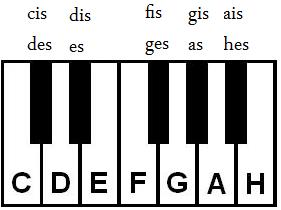
\includegraphics[width=0.4\linewidth]{obrazky/klaviatura.jpg}\\[1pt]  
    \caption{Přehledné uspořádání tónů a půltónů v oktávě \cite{orientaceNaKlaviature}}    
    \label{obrazekRozlozeniKlaviatury}
\end{figure*}

\section{Rytmus}
V melodii hudebních skladeb se málokdy vyskytují tóny a noty pouze jediného druhu.
Zpravidla se střídají dlouhé a krátké tóny, přízvučné a nepřízvučné.
Kolem přízvučného (silněji hraného) tónu se vyskytuje skupina delších a kratších tónů.
Tyto tvoří rytmický útvar a opakování rytmických útvarů udává rytmus.

\par
Rytmus je patrný především v hudbě určené pro tanec.
Mezi oblíbené tance s nápadnými rytmy patří například česká polka,
valčík a moderní tango. 
Některé tance a rytmy jsou spíše regionálního charakteru, 
mezi ně řadíme polské tance polonéza a mazurka, maďarský čardáš, či španělské bolero.
Složitými rytmy pak vynikají písně moravské a slovenské.
Rytmus je podle některých
\footnote{\uv{Na počátku byl rytmus} -- Hans Bülow} 
nejpodstatnější složkou hudby.
To je patrné především v hudbě národů na nízkém stupni kultury,
kde rytmy určené bicími nástroji, doplněné tleskáním a podupáváním,
zaujímají přední postavení tamní hudby.
\cite{cmiral}

\section{Stupnice a tónina}
\label{stupnice}

Stupnice je postupná řada tónů v rozsahu jedné oktávy.
Při poslechu je zřejmé, že jednotlivé stupně mezi sebou nemají konstantní vzdálenost.
\cite{kofron}
Některé dvojice dělí půltón čili malá sekunda, 
jiné větší krok (celý tón), velká sekunda.
Ta je rovna vzdálenosti dvou půltónů.
Vzdálenosti jednotlivých stupňů jsou dány pravidly.
\cite{cmiral}
Stupnice je možné rozdělit podle vzdáleností do několika kategorií.

\begin{enumerate}
	\item diatonické
	\begin{enumerate}
        \item staré (církevní)
        \item moderní (durové, mollové)
    \end{enumerate}
	\item chromatické
	\begin{enumerate}
        \item chromatické
        \item alterované
    \end{enumerate}
	\item exotické
	\begin{enumerate}
        \item cikánská
        \item pentatonická (čínská)
        \item celotónová
    \end{enumerate}
\end{enumerate}

V diatonických stupnicích jsou od sebe stupně vzdáleny jak o celé tóny, tak o půltóny.
V chromatických pak pouze o půltóny.
Exotické stupnice se od předchozích liší zvláštním uspořádáním stupňů.
\cite{kofron}
\par

Stupnici lze vytvořit od libovolného tónu.
V praxi se však používají jen ty, 
v nichž se uplatňují odvozené tóny nanejvýš dvakrát zvýšené nebo snížené.
Výchozí tón stupnice je jejím základním tónem a podle něj se stupnice jmenuje.
Například stupnice G dur začíná tónem \emph{g}, fis moll tónem \emph{fis}.
Rozdělení dur nebo moll se určuje podle vzdáleností mezi jednotlivými stupni.
\cite{zenkl}
Durové stupnice označujeme velkým písmenem, mollové malým.
Jednotlivé stupně stupnice se značí římskými číslicemi.
Mimo to má každý stupeň svůj funkční název:
\cite{kofron}

\begin{enumerate} [label=\Roman*]
    \item tónika
    \item supertónika (super = nad) nebo střídavá dominanta
    \item vrchní medianta
    \item subdominanta (spodní dominanta)
    \item dominanta (dominující, vládnoucí tón)
    \item spodní medianta
    \item citlivý tón - tíhne k půltónovému pokračování k tónice
\end{enumerate}
\par

Tóniny a stupnice mají stejné základní tóny a od toho také jména.
Opět, například pokud je tónina G dur, pak jejím základním tónem, tónikou je tón \emph{g}.
Tónina je volné pořadí tónů stupnice tvořící hudbu.
Není nutné, aby byly použity všechny tóny stupnice, 
ale jejich uspořádání musí dát vyniknout tónice.
Tónika se určuje sluchem pomocí tonálního cítění.
Velmi často melodie tónikou začíná nebo se k ní vrací.
V závěru melodie bývá tónika uplatňována nejčastěji.
V takovém případě působí melodie přesvědčivě uzavřena 
a posluchač necítí potřebu dalšího pokračování.
\cite{zenkl}
\par

\subsection{Durové stupnice}
Základní durovou stupnicí je C dur (c, d, e, f, g, a, h, c).
Durové, neboli tvrdé stupnice jsou charakteristické III. stupněm,
který s I. stupněm tvoří interval velké tercie.
Jinými slovy, první a třetí tón stupnice jsou vzdáleny dva celé tóny.
Vzdálenost mezi jednotlivými stupni durové stupnice jsou dva celé tóny, 
půltón, tři celé tóny, půltón.
$$ 1 - 1 - 1/2 - 1 - 1 - 1 - 1/2 $$
Půltóny jsou tedy mezi III.--IV. a VII.--VIII. stupněm.
Pro stupnice začínající od jiného základního tónu než \emph{c} 
je potřeba pomocí posuvek (viz část \ref{kapitolaPosuvky}:Posuvky) 
upravit vzdálenosti mezi jednotlivými stupni tak,
aby byly intervaly uspořádány jako ve stupnici C dur.
Takové stupnice  se jmenují transponované, je jich dohromady 14.
Sedm s křížky a sedm s béčky.
\cite{kofron}
\par

Při tvoření transponovaných durových stupnic s křížky 
se začíná od základní stupnice C dur (bez křížků i béček).
Následující stupnice (s $n$ křížky) začíná od pátého stupně té předchozí (s $n-1$ křížky).
Od tohoto tónu se opíše předchozí stupnice 
a předposlední VII. stupeň se zvýší jedním křížkem.
Nová stupnice má tedy o jeden křížek navíc.
Takto mohou vzniknout v pořadí následující stupnice: 
G dur (jeden křížek), D dur, A dur, E dur, H dur, Fis dur a Cis dur (sedm křížků).
Křížky v předznamenání stupnic jsou v tomto pořadí:
fis, cis, gis, dis, ais, eis, his.
Tento způsob tvoření stupnic se nazývá \emph{postup v kvintovém kruhu}.
\cite{kofron}
\par

Durové stupnice s béčky se vytvářejí podobně.
Opět se začíná od C dur, ale nyní se nová, 
následující stupnice (s $n$ béčky) opíše od čtvrtého stupně předchozí (s $n-1$ béčky)
a v nové stupnici se sníží jedním béčkem čtvrtý tón.
Tímto způsobem vznikají stupnice:
F dur (jedno bé), B dur, Es dur, As dur, Des dur, Ges dur, Ces dur (sedm bé).
Béčka v předznamenání jsou v tomto pořadí:
b, es, as, des, ges, ces, fes.
Způsob tvoření stupnic s béčky se nazývá \emph{postup v kvartovém kruhu}.
\cite{kofron}
\par

\subsection{Mollové stupnice}
Každá durová stupnice má svou paralelní mollovou, měkkou stupnici.
Ty mají při poslechu poněkud smutnější, tesklivější ráz.
Mollové stupnice se tvoří od VI. stupně durové stupnice.
Intervaly mezi stupni zůstávají nezměněny.
Například od stupnice C dur je odvozena základní mollová stupnice \emph{a} moll.
Vzdálenosti mezi stupni jsou $1 - 1/2 - 1 - 1 - 1/2 - 1 - 1$.
Stejně jako u durových stupnic lze odvozovat jiné, 
následující stupnice s křížky a béčky.
Následující stupnice s křížkem začíná na V. stupni a zvyšuje se II. stupeň.
Takto vzniknou stupnice e moll (jeden křížek), h moll, fis moll, cis moll, gis moll, dis moll a ais moll (sedm křížků).
Nová stupnice s bé začíná na IV. stupni a sníží se VI. stupeň.
Postupně vzniknou stupnice d moll (jedno bé), g moll, c moll, f moll, b moll, es moll, as moll (sedm bé).
\cite{kofron}
\par

\subsection{Akordy}
Akord je souzvuk alespoň tří různých tónů.
Pro tóny akordů platí určitá pravidla.
Pokud současně zní jiné tóny, pak spolu neladí.
Vztahem jednotlivých souzvuků se zabývá harmonie.
Při souznění všech tónů akordu najednou se jedná o harmonický akord.
Pokud jsou tóny zahrány po sobě, pak jde o melodický rozklad akordu.
Akordy lze třídit podle různých hledisek.
\cite{zenkl}

\begin{itemize}
    \item Podle počtu tónů: trojzvuky, čtyřzvuky, pětizvuky, vícezvuky
    \item Podle stavby: složené z tercií, z kvart
    \item Podle zvukového působení: konsonantní, disonantní
    \item Podle tvaru: základní, obraty akordu
\end{itemize}

Tercie je interval dvou tónů a dělí se na malou a velkou tercii.
Velká tercie je interval mezi prvním a třetím tónem durové stupnice 
a má tedy čtyři půltóny.
Malá tercie je také interval mezi prvním a třetím tónem, nyní ale mollové stupnice.
Má tedy pouze tři půltóny.
\cite{zenkl}
\par

Nejčastěji používané akordy jsou ty složené právě z tercií.
Pro vznik akordu je potřeba vedle sebe položit alespoň dvě tercie,
které dohromady tvoří kvintakord, 
kde interval mezi prvním a posledním tónem tvoří kvintu.
Přidáním další tercie vzniká septakord, ze čtyř za sebou pak nónový akord.
Změnou pořadí tónů akordu (například posunutím základního tónu o oktávu) 
vznikne obrat akordu.
\cite{zenkl}
\par

Kvintakordy se tedy tvoří z durových nebo mollových stupnic.
Jakost tercií v akordu dává jeho druh.
Durový akord se skládá ze spodní velké tercie a z horní malé.
Mollový ze spodní malé a horní velké.
Dále je možné použití dvou stejně velkých tercií.
Tak vzniká zvětšený nebo zmenšený kvintakord 
složený ze dvou velkých, respektive malých tercií.
\cite{kofron}
Pro akordy se vžila stejná pravidla jako pro stupnice, respektive tóniny.
Durové se zapisují velkým písmenem, mollové malým.
Tak jako stupnice, také durové akordy znějí vesele.
Mollové pak smutně, snížené až stísněně a zvětšené ostře, jasně.
\cite{cmiral}
Příkladem může být akord C dur složený z tónů \emph{c-e-g} 
nebo a moll z tónů \emph{a-c-e}.
\par

Kvintakordy dur a moll jsou konsonantní.
Svým zněním plně uspokojují posluchače a nevyžadují dalšího postupu (rozvedení hudby).
Naopak zvětšené nebo zmenšené jsou disonantní 
a je zvykem je dále rozvést (pokračovat) jiným, konsonantním akordem.
\cite{cmiral}

\subsection{Funkce akordů}
Harmonie se, kromě stavby akordů, zabývá také jejich uplatněním v hudbě.
Základním pojmem je harmonická funkce akordu.
Tedy význam akordu ve skladbě ve vztahu k její hlavní tónině.
Harmonie úzce souvisí s tóninou.
V durových i mollových tóninách existují tři základní harmonické funkce: 
tónika, dominanta, subdominanta.
Tónika je kvintakord postavený na I. stupni, dominanta na V. a subdominanta na IV. stupni.
Za povšimnutí stojí, že mají stejné názvy jako některé stupně  
(viz část \ref{stupnice}).
Na každém stupni durové, popřípadě mollové stupnice je totiž možné postavit kvintakord.
Každá stupnice je tak vybavena sedmi kvintakordy 
(osmý je stejný jako první).
Akordy na vedlejších stupních (II., III., VI., VII.)
vyjadřují také tyto harmonické funkce, ale jiným způsobem.
Pomocí nich je možné akordy hlavních stupňů zastupovat
a tímto způsobem obohatit harmonický doprovod písně.
\cite{kofron,zenkl}
\par

Hlavní akordy mají stejný tónorod jako tónina.
V durové tónině jsou durové, v přirozené mollové jsou mollové.
Avšak někdy se v mollové tónině využívá harmonická mollová stupnice,
která má zvýšený VII. stupeň.
U takových stupnic je pak dominanta durová.
\cite{kofron}
\par

Funkčnost akordů vyjadřuje snahu akordu po pohybu, jeho pohybovou energii.
Funkční značky (tónika, dominanta, subdominanta, \dots) 
vyjadřují smysl a celkový význam akordu.
Například, pokud po přehrání stupnice C dur zazní její tónický kvintakord,
pak má posluchač dojem klidu.
Ovšem při zaznění dominantního kvintakordu je cítit snaha po dalším postupu.
Člověk má dojem, jako by tóny dominanty chtěly stoupat vzhůru.
Pro uklidnění je po dominantě potřeba zahrát tóniku.
Ta je akordem klidu, harmonickým centrem tóniny.
\cite{kofron}
Ve většině písní také slouží jako přesvědčivý závěr.
\cite{zenkl}
Naopak dominanta, protože obsahuje citlivý tón stoupající, 
je akordem pohybu a snaží se stoupat k tónice.
\cite{kofron}
Subdominanta je také akordem pohybu 
a má snahu je od tóniky odklonit k dominantě.
\cite{zenkl}
Pokud je subdominanta mollová, pak také obsahuje citlivý tón, 
nyní ale klesající.
Tyto tři hlavní kvintakordy velmi často stačí 
k harmonizaci jednoduchých a krátkých skladeb.
\cite{kofron}
Harmonizace moderních či více uměleckých skladeb využívá mimo jiné
také kvartové akordy, nepravidelné souzvuky,
akordy zhuštěné sekundami (interval mezi I. a II. stupněm) nebo
kombinace tonálně uvolněných akordů, případně až atonálních.
Chvilková disharmonie skladby také nemusí být na škodu,
jedná-li se o umělecký záměr skladatele.
\cite{zenkl}
\par

\section{Notopis}
Alfabetické znaky nejsou pro značení tónů dostatečné, protože popisují pouze výšku tónu.
Pro hru na hudební nástroj nebo skládání hudby je potřeba specifikovat také zbývající vlastnosti.
Po staletí trvajícím vývoji se ustálil a používá se notopis.\par

\subsection{Notová osnova}
Základem jsou noty a notová osnova, kterou tvoří pět linek a čtyři mezery.
Noty se zapisují na linky i do mezer.
Takto lze zapsat pouze devět not.
Notovou osnovu lze však rozšířit pomocnými linkami nad, popřípadě pod notovou osnovou. 
Pomocné linky se zapisují pouze tak dlouhé, jak je nezbytně nutné.
Pro snadnou orientaci v osnově se v praxi počítají linky a mezery směrem nahoru (s výjimkou pomocných linek pod osnovou). 
Linky a mezery se počítají zvlášť. 
První mezera je mezi první a druhou linkou.\par

\begin{figure*}[h]\centering
    \centering
    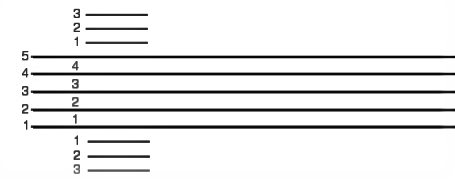
\includegraphics[width=0.5\linewidth]{obrazky/notovaOsnova.png}\\[1pt]  
    \caption{Číslování notové osnovy}    
    \label{obrazekNotovaOsnova}
\end{figure*}

\subsection{Noty}
Samotné noty jsou písemné značky pro tóny.
Tvar noty vyjadřuje délku noty a pozice v notové osnově její výšku.
Nota se skládá z několika částí.
Hlavička určuje pozici noty, a může být buď vyplněná , nebo nevyplněná . 
Nožka opět buď může být, a nebo nemusí . 
Pokud nota nožku má, pak ji, u not na třetí, prostřední lince a vyšších, píšeme směrem dolů ,
a naopak u nižších not směrem nahoru.
I toto pravidlo má ovšem nějaké výjimky.
Poslední částí noty je praporec, těch může mít nota nula až čtyři .
Pokud je za sebou víc not s praporci, lze je spojit, a praporce nahradit trámci.
V hudbě se používají tyto základní noty:

\begin{figure*}[h]\centering
    \centering
    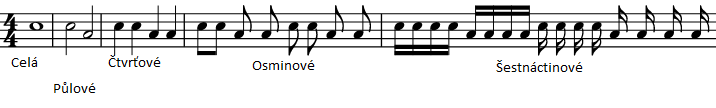
\includegraphics[width=0.8\linewidth]{obrazky/druhyNot.png}\\[1pt]  
    \caption{Noty ve čtyř čtvrťovém taktu.}    
    \label{obrazekNoty}
\end{figure*}

Podle názvů not je zřejmé, že nota celá má délku dvou půlových not, 
čtyř čtvrtinových osmi osminových a tak dále.
Nejbližší nižší nota má délku poloviční a nejbližší vyšší dvojnásobnou.
\par

\subsection{Klíče}
Jména (výšky) not v osnově jsou určeny takzvaným klíčem, 
který se píše vždy na začátek každého řádku.
Klíčem se označuje pozice a jméno jedné noty 
a od ní se pojmenují ostatní v pořadí, 
přičemž pojmenování se řídí hudební abecedou.
Tvary klíčů se vyvinuly z písmen not, jejichž linku označují.
V současné době se používají čtyři klíče(viz obrázek \ref{obrazek4Klice}), 
a to G-klíč (houslový), F-klíč (basový) a dva C-klíče (altový a tenorový).

\begin{figure*}[h]\centering
    \centering
    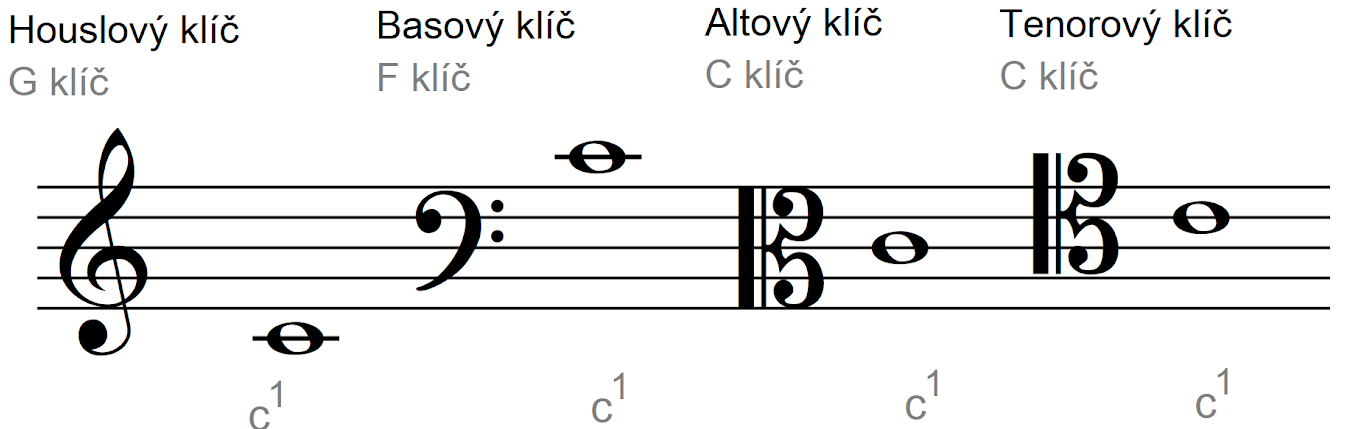
\includegraphics[width=0.6\linewidth]{obrazky/Klíče.png}\\[1pt]  
    \caption{Hudební klíče s příslušnou pozicí noty $c^1$}    
    \label{obrazek4Klice}
\end{figure*}

Houslový klíč označuje notu $g^1$ na druhé lince.
Basový určuje malé f na čtvrté lince, altový $c^1$ na třetí 
a tenorový také $c^1$ na čtvrté lince.
Basový klíč je nejvhodnější pro notaci hlubokých tónů 
a houslový k notaci vysokých.
Tyto dva klíče se používají nejčastěji. 
Pro orientaci v těchto klíčích je dobré vědět, že
tón $c^1$ se v houslovém klíči nachází na první spodní pomocné lince, 
a v basovém se nachází na první horní pomocné lince.
\cite{cmiral,zenkl}
\par

\subsection{Pomlky}
Kromě značení tónů je v hudbě potřeba zaznačit také odmlky,
tedy místa kdy má být ticho.
Ticho se značí zvláštními značkami, pomlkami v notovém zápise 
a mají stejné hodnoty jako noty.
Délka pomlky je opět, jako u not, 
dána tvarem (viz obrázek \ref{obrazekPomlky}).
Celá pomlka značí pomlku na jakýkoliv celý takt.
\cite{cmiral,zenkl}

\begin{figure*}[h]\centering
    \centering
    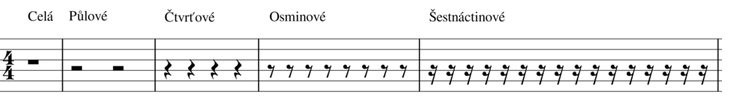
\includegraphics[width=0.8\linewidth]{obrazky/pomlky.png}\\[1pt]  
    \caption{Pomlky ve čtyř čtvrťovém taktu}    
    \label{obrazekPomlky}
\end{figure*}

\subsection{Posuvky}
\label{kapitolaPosuvky}
Samotné noty značí pouze základní tóny.
Pokud chceme, aby nota značila zvýšený tón, 
je potřeba před ni (na její linku, nebo mezeru) napsat křížek ($\sharp $).
Je-li před notou béčko ($\flat $), pak nota značí tón snížený.
Posuvky lze psát buď přímo před notu, kterou chceme alterovat, 
nebo na začátek každého řádku, pak předznamenává tóninu.
Platnost posuvky před notou je do konce taktu.
Je možné ukončit účinnost dříve, odrážkou ($\natural $).
Zde ovšem platí, že pokud byla posuvka na začátku řádku, 
odrážka platí do konce taktu.
\cite{cmiral,zenkl}

\subsection{Takty}
Noty a pomlky se řadí do krátkých úseků, 
ze kterých se skládá celá hudební skladba.
Tyto úseky nazýváme takty.
V notové osnově jsou od sebe odděleny tenkými svislými čarami.
Pokud je skladba pro více nástrojů a je notována na více řádků, 
pak protíná taktová čára všechny řádky.
Na konci skladby je taktová čára doplněna ještě jednou silnější čarou. 
Takty dělíme na doby -- stejně dlouhé časové úseky.
Podle počtu dob jsou takty dvoudobé až třídobé.
Doby mohou být půlové, osminové, nejčastěji však čtvrťové.
První doba je vždy přízvučná, hraje se silněji.
Ostatní doby jsou hrány bez přízvuku, 
pokud nejsou opatřeny zvláštní značkou~($>$) nad notou.
Takto popsané jsou takty jednoduché.
Spojením dvou jednoduchých taktů vzniká takt složený.
Složené takty mají dva přízvuky.
Silnější na začátku taktu, a o něco slabší tam, 
kde by začínal druhý jednoduchý takt.
\par

Součet hodnot not v každém jednom taktu se musí rovnat počtu dob taktu.
Čili například v jednom  dvoučtvrťovém taktu 
může být jedna nota půlová (má dvě doby), 
dvě noty čtvrťové, jedna čtvrťová a dvě osminové, a tak dále.
To, jaký má skladba takt, zjistíme na začátku skladby, kde je zapsán zlomek.
Čitatel uvádí počet dob a jmenovatel hodnotu počítané doby.
V průběhu skladby může dojít ke změně taktu.
Tuto změnu značíme taktovým označením hned za taktovou čáru, 
kde změna začíná.
Čtyřčtvrťový takt se většinou nazývá celý 
a místo zlomku je značen velkým písmenem C.
\cite{cmiral,zenkl}

\chapter{Data}
% ABC, MIDI, GUIDO ... viz NOTES.md
V této části jsou popsány vstupní data.
Zadání specifikuje některý ze standardizovaných formátů.
Jedním z nich je MIDI.
Tento formát je popsán v první části této kapitoly.
Veškerá data pro tuto diplomovou práci pochází z webu \url{https://www.hooktheory.com/}.
Ten obsahuje takzvanou Theorytab DB, databázi přepisů známých písniček.
Přepisy obsahují melodii, harmonii ve formě harmonické funkce a odkaz na písničku na \url{www.youtube.com}
Jejich podobu a převedení do MIDI popisuje druhá část.

\section{MIDI soubory}
MIDI (Musical Instrument Digital Interface) je volně přístupný standard,
který specifikuje hardware i software 
pro digitální komunikaci hudebních nástrojů,
sekvencerů, počítačů, mixérů, 
a dokonce i jevištní techniky, jako jsou reflektory a lasery.
\cite{MIDI_tutorials}
\par

Standardní MIDI soubor (zkráceně SFM) je formát binárních souborů 
určených pro uložení a přenos hudebních dat mezi zařízeními.
Soubory v tomto formátu lze rozeznat pomocí \emph{.mid} přípony.
Oproti ostatním formátům pro uložení zvuku 
SFM neukládají digitalizovaný zvuk,
ale parametry použitých nástrojů, informace o tempu, kanálech, 
jednotlivé noty uložené jako kombinace (čas, hodnota, rychlost) 
a další MIDI události.
Data z těchto souborů jsou načteny do nějakého přehrávače 
a výsledný zvuk je vytvořen připojeným sound-enginem.
\cite{MIDI_tutorials,Neznamy_aboutMIDIFiles}
\par

Data v SFM jsou uložena v blocích.
Každý z těchto bloků začíná čtyřbajtovým textovým označením 
a čtyřbajtovou délkou datového bloku udávající počet bajtů.
Ihned po délce začíná datová část o délce zadané v hlavičce.
Za datovou částí začíná buď další blok, nebo konec souboru.
\cite{MIDI_tutorials,Back_SMF_Specif}
\par

Soubory MIDI mají dva druhy bloků. 
Hlavičkový blok poskytuje informace vztahující se k celému souboru.
Bloky stopy obsahují proudy MIDI dat až šestnácti MIDI kanálů.
MIDI soubor vždy začíná hlavičkovým blokem 
a je následován jedním, nebo více bloky stop.\cite{Back_SMF_Specif}

\begin{itemize} [label={}]
    \item MThd <délka hlavičky>
    \item <data hlavičky>
    \item MTrk <délka stopy>
    \item <data stopy>
    \item MTrk <délka stopy>
    \item <data stopy>
    \item \dots
\end{itemize}

\subsection{Hlavička}
Blokem hlavičky začíná každý MIDI soubor a obsahuje jeho základní popis.
Je uvozen typem bloku, čtyřmi ASCII znaky "MThd" 
a 32bitovou reprezentací čísla 6 (délka bloku). 
Začátek SMF je tedy pevně daný, 
a takový soubor lze na první pohled rozeznat začínající sekvencí 
\emph{0x4D 54 68 64 00 00 00 06}. 
Datovou část tvoří tři 16bitové slova.
První z nich specifikuje formát, celkovou organizaci souboru.
Tím je myšleno uspořádání uložených stop.
Jsou zde tři možnosti:

\begin{enumerate}\addtocounter{enumi}{-1}
    \item soubor obsahuje jedinou více-kanálovou stopu
    \item několik souběžných stop
    \item několik nezávislých stop
\end{enumerate}

Formát 0 je nejrozšířenější a je podporován i nejjednoduššími programy 
a hardware.
\cite{Back_SMF_Specif}
Formát 1 obsahuje jednu nebo více vertikálně synchronních stop.
Jinými slovy, při přehrávání takového souboru 
začnou všechny stopy ve stejný čas 
a mohou reprezentovat různé části písničky.
V posledním, asynchronním formátu nemusí stopy nutně začínat ve stejnou dobu
\cite{Neznamy_aboutMIDIFiles}.
Tento formát je nejméně používaný
\cite{MIDI_tutorials}.
\par

Dalším slovem hlavičky je počet stop.
Ten je u nultého formátu vždy roven jedné.
Poslední část definuje kódování času, 
které může být zadáno dvěma způsoby.
Ty jsou dány prvním bitem slova.
Pokud je bit nulový, 
pak zbývající bity reprezentují počet "tiků" generátoru hodin, 
které se vlezou do jedné čtvrťové noty.
Pokud je bit nastaven na 1, 
pak je čas vyjádřen jako rozdělení vteřin podle SMPTE standardu
a MIDI Time Codu.
\cite{Back_SMF_Specif}
Filmovým průmyslem vytvořený SMPTE, mimo jiné, 
definuje čtyři různé snímkovací frekvence.
Je podle něj možné rozdělit vteřinu na 24, 25, 29 nebo 30 snímků.
Pro hudební účely je však potřeba ještě jemnější rozlišení.
Každý snímek je tedy dále možné rozdělit na "sub-snímky".
\cite{Neznamy_aboutMIDIFiles}
Bity 14 až 8 časového kódování udávají počet SMPTE snímků za vteřinu 
a zbývající část je rozlišení jednoho snímku.
Pro představu,
při časování událostí na milisekundy je potřeba nastavit 25 SMPTE snímků,
a rozlišení 40, neboť $ 40 * 25 = 1000 $ "sub-snímků" za vteřinu, 
stejně jako milisekund. 
\cite{Back_SMF_Specif}
\par

\subsection{Stopy}
Každý MIDI soubor obsahuje nejméně jeden blok stopy.
Ten obsahuje parametry použitých nástrojů, jednotlivé noty skladby, 
ale také různé textové informace jako název skladby nebo její text.
Za identifikátorem bloku "MTrk" a jeho délkou 
následuje posloupnost MIDI událostí
ve tvaru časový přírůstek, stavový bajt, datové bajty.
\cite{Back_SMF_Specif}
\par

Časový přírůstek (deltatime) značí počet "tiků" od předchozí události.
Tato hodnota má proměnnou délku.
Její formát umožňuje velkým číslům využít tolik bajtů, 
kolik potřebují bez toho,
aby malá čísla plýtvala místem a plnila jej nulami.
Hodnoty jsou kódovány do 7-bitových bajtů 
a osmý, nejvýznamnější bit je nastaven na jedničku.
Pokud je bajt poslední v posloupnosti, pak na nulu.
Celý deltatime by však ideálně neměl přesáhnout 4 bajty.
\cite{Neznamy_aboutMIDIFiles}
První událost stopy, nebo dvě současné události 
mají časový přírůstek roven nule.
\cite{Back_SMF_Specif}
\par

Za časem následuje MIDI zpráva tvořená stavovým bajtem 
a až dvěma datovými bajty.
Stavový bajt má vždy nejvýznamnější bit jedničku,
zatímco datové mají nulu.
Pokud je stav vynechán a za deltatime následují datové bajty, 
pak je lze poznat právě nulovým nejvyšším bitem.
Je několik druhů stavů a je možné je rozdělit na 
kanálové zprávy (Channel Messages) 
a systémové zprávy (System Messages).
Kanálové zprávy se vztahují k specifickému kanálu.
Jeho číslo je zapsáno ve spodním půlbajtu stavu zprávy.
Tedy například \emph{0x91} představuje změnu stavu na kanále jedna.
V proudu je možné rozeznat dva druhy kanálových zpráv.
Channel Voice Message přenáší hudební produkci 
a tvoří většinu provozu MIDI proudu.
To jak na tyto zprávy budou přijímající nástroje reagovat 
je dáno Channel Mode zprávami.
Systémové zprávy jsou buď 
určeny všem přijímačům v systému (System Common Message),
použity pro synchronizaci hodin MIDI komponent (System Real Time Message), 
nebo použity pro přenos dat mezi komponenty jednoho výrobce 
(System Exclusive Message). 
\cite{Back_SMF_Specif}
\par

Aktivace a vypuštění jedné noty je v MIDI považováno za dvě rozdílné události.
Jsou to kanálové zprávy \emph{Note on} a \emph{Note off},
z nichž první rozezní daný tón určitou silou a druhý ji utiší.
Přijetí \emph{Note On} rozeznáme stavovým bajtem \emph{0x9k}, 
kde \emph{k} určuje na kolikátém kanále bude nota znít.
Následuje datový bajt s číslem rozeznívané noty.
Čísla not jsou odvozena od středního, jednočárkového c, 
kterému je přiřazena hodnota 60 (viz tabulka \ref{tableMIDINotes}).
Z toho vyplývá, že subkontra oktáva je nultá a čtyřčárková je sedmá.


\begin{table}[]
    \centering
    \begin{tabular}{l|llllllllllll}
        \multirow{2}{*}{\textbf{Oktáva}} & \multicolumn{12}{l}{\textbf{Čísla not}}                                                                                                                             \\
                                         & \textbf{C} & \textbf{C\#} & \textbf{D} & \textbf{D\#} & \textbf{E} & \textbf{F} & \textbf{F\#} & \textbf{G} & \textbf{G\#} & \textbf{A} & \textbf{A\#} & \textbf{B} \\ \hline
        \textbf{-1}                      & 0          & 1            & 2          & 3            & 4          & 5          & 6            & 7          & 8            & 9          & 10           & 11         \\
        \textbf{0}                       & 12         & 13           & 14         & 15           & 16         & 17         & 18           & 19         & 20           & 21         & 22           & 23         \\
        \textbf{1}                       & 24         & 25           & 26         & 27           & 28         & 29         & 30           & 31         & 32           & 33         & 34           & 35         \\
        \textbf{2}                       & 36         & 37           & 38         & 39           & 40         & 41         & 42           & 43         & 44           & 45         & 46           & 47         \\
        \textbf{3}                       & 48         & 49           & 50         & 51           & 52         & 53         & 54           & 55         & 56           & 57         & 58           & 59         \\
        \textbf{4}                       & 60         & 61           & 62         & 63           & 64         & 65         & 66           & 67         & 68           & 69         & 70           & 71         \\
        \textbf{5}                       & 72         & 73           & 74         & 75           & 76         & 77         & 78           & 79         & 80           & 81         & 82           & 83         \\
        \textbf{6}                       & 84         & 85           & 86         & 87           & 88         & 89         & 90           & 91         & 92           & 93         & 94           & 95         \\
        \textbf{7}                       & 96         & 97           & 98         & 99           & 100        & 101        & 102          & 103        & 104          & 105        & 106          & 107        \\
        \textbf{8}                       & 108        & 109          & 110        & 111          & 112        & 113        & 114          & 115        & 116          & 117        & 118          & 119        \\
        \textbf{9}                       & 120        & 121          & 222        & 123          & 124        & 125        & 126          & 127        & \multicolumn{4}{l}{}                                 
    \end{tabular}
    \caption{Čísla všech MIDI not po oktávách \cite{Back_SMF_Specif}}
    \label{tableMIDINotes}
\end{table}

MIDI bylo původně určené pro klávesové nástroje, 
druhý datový bajt je tedy pojmenován rychlost (zmáčknutí klapky),
ale ve výsledku určuje to, jak hlasitě (s jakou amplitudou) bude tón znít oproti ostatním.

Pro ztlumení znící noty slouží zpráva \emph{Note Off} označená bajtem \emph{0x8k}.
Stejně jako při rozeznění je potřeba vědět, o jakou notu se jedná.
A také v tomto případě je ve zprávě obsažena rychlost (puštění klapky), 
která je ale ve většině případech ignorována.
\cite{MIDI_tutorials}

\section{Databáze Hooktheory}
\label{hooktheoryDB}
Data k projektu byla získána ve formě SQLite
\footnote{\url{https://sqlite.org/index.html}} databáze.
Tato databáze obsahuje záznamy o písničkách extrahovaných z webu \url{https://www.hooktheory.com/}.
Velikost databáze je $32.7$MB ($34 334 720$B)

Databáze se skládá z několika tabulek.
Základní tabulkou je \emph{url2id}, 
která mapuje webový odkaz písničky na identifikátor (dále jen id) písničky v databázi.
Odkazy v databázi jsou zkrácené, a neobsahují doménové jméno webu.
Pokud je písnička na webu 
například pod odkazem \emph{https://www.hooktheory.com/theorytab/view/the-beatles/hey-jude},
pak v databázi je pouze část \emph{/theorytab/view/the-beatles/hey-jude}.
\par

Kvůli autorským právům nelze přepsat celou písničku.
Místo toho uživatelé Hooktheory přepisují pouze její unikátní části, 
ne delší než 30 vteřin.
Jména úseků jsou například úvod (Intro), sloka (Verse), nebo refrén (Chorus).
\cite{ht_guide}
Další tabulka v databázi spojuje písničky s jejími částmi.
Její jméno je \emph{id2parts} a mapuje id písniček na id všech jejích částí.
Tabulka \emph{parts} obsahuje informace o těchto částech.
Jejími sloupci jsou:

\begin{itemize}
    \item id - identifikátor části
    \item name - jméno příslušné písničky
    \item songkey - tónina části
    \item xml - BLOB\footnote{Binary Large Object} obsahující komprimovaný XML soubor s dalšími informacemi
    \item json - nic neobsahující sloupec
\end{itemize}

Kořenový uzel XML souboru z databáze obsahuje dva potomky -- meta a sections.
Meta obsahuje základní informace popisující část písničky.
Jedná se o jméno autora písničky, jednoznačné jméno části (například Hey Jude Chorus),
počet dob v taktu, počet dob za minutu (BPM\footnote{z anglického Beats per minute}),
opět tónina, mód části,
odkaz na Youtube a časy začátku a konce dané části v Youtube videu.
\par
Sections obsahuje uzel pojmenovaný podle názvu části písničky 
(Intro, Verse, Chorus\dots).
Části písniček jsou rozděleny na segmenty.
Uvnitř segmentů jsou kategorie, 
které dále obsahují samotné noty (uzel notes) a akordy (uzel chords). 
Každá nota má několik vlastností.
První čtyři se týkají času.
Pro orientaci uvnitř taktu slouží \emph{start\_beat}, 
jenž značí, v kolikáté době taktu nota začíná.
Tento čas je počítán od jedničky.
Takže například nota začínající znít v první době taktu
má \emph{start\_beat} nastaven na 1.
Takt, ve kterém je nota aktivní označuje \emph{start\_measure}.
Obě tyto vlastnosti dává dohromady vlastnost \emph{start\_beat\_abs},
která udává absolutní počet dob od začátku písničky, 
po začátek noty.
Délku noty v dobách je zapsána v \emph{note\_length}.
Následují dvě vlastnosti týkající se výšky tónu.
\emph{Scale\_degree} nabývá hodnot 1 až 7 podle použitého stupně tóniny,
popřípadě \emph{rest}, pokud je místo noty použita pomlka.
Oktávu noty udává \emph{octave} jako počet oktáv, 
které je nutno přičíst k oktávě s notou C60 (viz tabulka \ref{tableMIDINotes})
Například \emph{octave} noty C60 je nula, 
noty C48 minus jedna a noty C72 plus jedna.
Poslední xml vlastností noty je redundantní \emph{isRest},
pravdivostní hodnota s jedničkou, pokud se jedná o pomlku. 
\par

Akordy jsou v xml popsány podobně jako noty.
Vlastnosti \emph{start\_beat}, \emph{start\_measure}, \emph{start\_beat\_abs}
a \emph{isRest} mají stejný význam.
Délku trvání akordu značí \emph{chord\_duration} stejně jako u not v počtu dob.
Zbývající vlastnosti popisují akord jako takový.
První tón akordu, a tedy i jeho název, 
je ukryt v uzlu se zkratkou \emph{sd},
nejspíš s anglického scale degree.
Stejně jako u not má tato vlastnost rozsah 1 až 7 podle stupně tóniny 
popřípadě \emph{rest}.
Vlastnost a zkratka \emph{fb} je z anglického figural bass, 
tedy číslovaný bas. 
Číslo ve vlastnosti značí, 
na kterém stupni se nachází základní tón akordu\cite{kofron}.
Zkratka \emph{sec} mění základní tóninu,
od které se počítá stupeň akordu (\emph{sd}).
Akord, ve kterém je vyměněna tercie za kvartu, případně sekundu,
se jmenuje suspended akord.
Pokud se jedná o tento akord, 
pak vlastnost \emph{sus} obsahuje řetězec \emph{sus4} v případě kvarty,
\emph{sus2} v případě sekundy, nebo \emph{sus42} v případě obou\cite{SimplifyingSuspended}.
Akord lze také vyměnit za akord z jiného modu.
Toto "vypůjčení" je zaznamenáno v uzlu \emph{borrowed}.
Složka \emph{alternate} značí akordy alterované, 
tedy akordy s jedním nebo více tóny alterovanými.
\cite{SzkanderaAlterovane}.
\par
Kromě těchto popsaných tabulek obsahuje databáze také další,
které popisují žánr písničky, 
nebo její metriky zavedené a vypočítané webem hooktheory.com.
Tato data ale nejsou vzata v úvahu, 
neboť s nimi nelze počítat ve standardních MIDI souborech.

\subsection{Převedení databáze na MIDI soubory}
Pro účely práce je nutné jednotlivé záznamy databáze
konvertovat na množinu MIDI souborů.
Proto jsem vytvořil skript \emph{dbToMIDI.py} v jazyce Python,
který sekvenčně dotazuje jednotlivé části písniček v databázi,
a pro každou vytvoří samostatný MIDI soubor.
Tyto soubory uloží do složky 
a pojmenuje ve formátu {<id písničky>\_\_part<id části>.mid}.
Cestu k databázi a jméno výstupní složky 
je nutno zadat jako vstupní parametry složky v tomto pořadí.
Pro práci s databází skript využívá knihovnu \emph{sqlite3}\footnote{https://docs.python.org/3/library/sqlite3.html}.
Data jako noty a akordy jsou v xml souboru, 
který je uložený v jednom ze sloupců.
Soubor xml je dekomprimován metodou \emph{decompress()} z knihovny 
\emph{zlib}\footnote{https://docs.python.org/3/library/zlib.html},
Pro extrakci těchto dat je využita knihovna \emph{lxml.etree}\footnote{https://lxml.de/}.
Manipulace s MIDI soubory je prováděna pomocí knihovny Mido\footnote{https://github.com/mido/mido}.
Každý záznam části písničky v databázi má, mimo jiné, 
xml uzel s notami a uzel s akordy.
Skript postupně projde nejprve všechny noty, a poté akordy,
a na základě poskytnutých dat vypočítá výšky tónů, čas začátku a čas konce.
S pomocí výsledných parametrů jsou vytvořeny \emph{mido.Message} objekty,
které abstrahují MIDI zprávy.
Tyto objekty jsou poté vloženy do dvou objektů \emph{mido.MidiTrack}.
Jeden slouží pro ukládání melodických not, a druhý pro harmonické akordy.
Z těchto stop je vytvořen \emph{mido.MidiFile} objekt, který zaštiťuje práci s MIDI souborem.
Některé záznamy písniček obsahují pouze akordy, nebo pouze noty, tedy melodii bez harmonie.
Soubor je na tento neduh otestován, a pokud obsahuje obě složky, pak je uložen.
Ty, kterým jedna z částí chybí uloženy nejsou.
Z celkového počtu $13 633$ je tímto způsobem odstraněno zhruba $1500$ částí písniček.
Celková velikost všech souborů je $9.57$MB ($10 042 700$B)

\chapter{Přehled přístupů automatické harmonizace}
\label{prehledPristupus}
Pojem automatická harmonizace melodie označuje disciplínu, která se zabývá tvorbou modelu, 
který dokáže vygenerovat harmonický doprovod k dané melodii.
Samotná harmonizace je složitý úkol, 
protože tu samou melodii můžeme harmonizovat mnoha různými způsoby.
Správná harmonie závisí na subjektivním pocitu, hudebním žánru a dalších faktorech.
V hudbě se ustálilo mnoho pouček a zákonů o tom, které akordy k sobě patří,
a jak na sebe navazují.
Často určují jemné nuance, či jsou podmíněny kulturním vlivem, 
což je pro stroj velmi obtížné zachytit.
\cite{YinCheng_comparativeStudy}
\par

V této kapitole bude představeno několik přístupů právě k automatické harmonizaci.

\section{Model založený na shodě šablon}
\label{shodaSablon}
Tento model nejdříve rozdělí všechny melodie z trénovací sady po polovinách taktů, 
a pro každý, takto vytvořený segment vytvoří profil výšky tónů 
(dále jen PCP\footnote{z anglického Pitch Class Profile}).
\cite{YinCheng_comparativeStudy}
PCP je dvanácti-dimenzionální binární vektor, 
kde každá složka reprezentuje přítomnost 
každého z dvanácti možných půltónů v daném půl-taktu.
\cite{fujishima}
PCP nového segmentu se porovná s těmi z trénovací sady
a spočítá se podobnostní skóre.
Nový segment je pak označen takovým akordem,
který měl jemu nejpodobnější segment v trénovací sadě -- s nejvyšším skóre.
Jestliže má nejvyšší skóre několik segmentů,
je výsledný akord vybrán náhodně s rovnoměrným rozložením pravděpodobnosti.
Označení akordu je opět ve formě PCP, a to tak,
že všechny tóny náležící akordu jsou nastaveny do 1.
\par

Nevýhodou tohoto modelu je, že určuje jednotlivé segmenty nezávisle bez toho,
aby bral v úvahu sousední akordy, nebo postup akordů ve skladbě.
\cite{YinCheng_comparativeStudy}

\section{Skryté Markovovy modely}
Jednou z nejpoužívanějších metod generování akordů a harmonizace melodie, 
před současným rozšířením hlubokého učení, byly skryté Markovovy modely 
(dále HMM \footnote{z anglického Hidden Markov Model}).
HMM jsou pravděpodobnostní nástroj, 
s jehož pomocí lze modelovat sekvence se skrytými proměnnými.
Označení akordů je považováno právě za skrytou proměnnou a 
HMM se snaží odhadnout nejpravděpodobnější sekvenci akordů
k daným notám melodie.
Na rozdíl od předchozího přístupu 
tento model bere v úvahu předcházející akordy.
\cite{YinCheng_comparativeStudy}

\section{Google Magenta}
\label{magenta}
Magenta je open-source výzkumný projekt založený Google Brain týmem.
Jedná se o soubor nástrojů a modelů hlubokého i posilovaného učení.
Zaměřuje se především na využití strojového učení jako nástroje
v kreativním procesu.
Projekt je distribuován pro Python a JavaScript.
Magenta.js je pouze API pro používání předtrénovaných modelů v prohlížečích.
Magenta pro Python je celá knihovna, která zahrnuje kromě předtrénovaných modelů
také nástroje pro manipulaci dat, trénování vlastních modelů a generování
nových výtvorů na jejich základě.
\cite{google_magentaHome} 
Vytvořené modely se zabývají generováním a modifikací hudebních 
a obrazových uměleckých dat.
Obrazové modely jsou například image\_stylization\footnote{https://github.com/magenta/magenta/tree/master/magenta/models/image\_stylization},
který vytvoří nový obraz na základě obsahu jednoho a stylu druhého\cite{dumoulin2017learned},
nebo sketch-rnn\footnote{https://github.com/magenta/magenta/tree/master/magenta/models/sketch\_rnn},
tedy rekurentní neuronovou síť, která se pokouší domalovat člověkem vytvořený náčrt,
popřípadě načrtnout obrázek dle zadané třídy\cite{ha2017neural}.
\par

Z hudebních modelů Magenta obsahuje Coconet, 
který doplňuje zadanou melodii o kontrapunkt, 
tedy o protihlas více melodií\cite{kofron, huang2017counterpoint}.
Rozdílem oproti klasickým algoritmům doplňující kontrapunkt
je oproštění od chronologického postupu od začátku skladby ke konci.
Naopak noty jsou generovány v jakémkoliv pořadí tak, 
že model opakovaně přepisuje a maže svou vlastní práci.
Při trénování model přijímá čtyřhlasou harmonii s náhodně odstraněnými notami,
a snaží se tento vstup rekonstruovat.
Na nižší úrovni je vstup tří dimenzionální pole, 
kde jedna z dimenzí vymezuje čtyřhlas, další číslo MIDI noty a poslední čas\footnote{V literatuře se pole s dimenzemi (MIDI nota, čas) nazývají pianoroll}.
Tento objekt je vstupem konvoluční neuronové sítě.  
Výstupem je objekt o stejné velikosti, 
nyní obsahující pravděpodobnosti not ve smazaných částech.
\cite{huang2017counterpoint}
Tento natrénovaný model lze vyzkoušet jako Google Doodle na \url{https://www.google.com/doodles/celebrating-johann-sebastian-bach}
\par
Jedním z dalších Magenta modelů, které se zabývá hudbou je méně propagovaný Polyphony RNN. 
Ten aplikuje jazykové modely ke generování polyfonní hudby za použití LSTM neuronových sítí
a je založen na projektu BachBot, který je popsán v \cite{Liang_AutomaticComposition}.
Na rozdíl od modelu Melody RNN, který také využívá jazykových modelů, 
Polyphony RNN dokáže pracovat s více souběžnými notami.
Tento model tedy pracuje také s vícehlasem.
Více-hlasý vstup je zde modelován jako jeden proud notových událostí se speciálními řídícími symboly.
Skladba je rozdělena na stejné časové úseky (stepy), 
a každý z úseků obsahuje seznam aktivních not.
Noty jsou v každém úseku seřazeny podle výšky (v MIDI formátu) 
a je popsán jejich vztah v závislosti k předchozímu stavu tónu(viz níže akord C trvající dva úseky).
\cite{google_git_polyphony}
\begin{verbatim}
START
NEW_NOTE, 67
NEW_NOTE, 64
NEW_NOTE, 60
STEP_END
CONTINUED_NOTE, 67
CONTINUED_NOTE, 64
CONTINUED_NOTE, 60
STEP_END
END
\end{verbatim}
Pro generování nové skladby potřebuje model tzv. primer, tedy pár not, 
použitých jako počátek skladby. 
Primer lze vložit ve třemi způsoby, a to jako počáteční akord,
počáteční melodie, nebo MIDI soubor.
Tento vstup lze vložit do modelu před generováním,
tedy ve vygenerované sekvenci vstup nebude, ale bude jím oblivněn.
Toto se hodí například pro ustanovení tóniny generované skladby.
Dále je možné použít vstup jako součást generované sekvence,
což je vhodné při harmonizaci již existující melodie.
\cite{google_git_polyphony}

\chapter{Strojové učení}
% rešerše strojového učení, jak funguje
Umělá inteligence dokázala relativně rychle řešit problémy, 
které jsou pro člověka intelektuálně náročné, 
ale jsou popsány formálními pravidly.
Avšak pro člověka intuitivní \"problémy\" lze jen s těží formálně popsat.
Strojové učení umožňuje počítači naučit se ze zkušeností
a porozumět světu v souvislostech.
Získáváním zkušeností je odbourán proces formálního zápisu veškerých vědomostí,
které jsou k řešení problému potřeba.
\cite{Goodfellow-et-al-2016}
Harmonizace melodie je někde na půl cesty mezi těmito extrémy.
Na jednu stranu popsána pravidly hudební nauky,
na stranu druhou nejsou pravidla zcela striktní 
a ponechávají skladateli volnou ruku.
\par

Strojové učení je v podstatě forma aplikované statistiky,
s důrazem na odhad složitých funkcí počítačem.
Většina algoritmů lze rozdělit do dvou kategorií --
učení s učitelem (supervised) 
a učení bez učitele (unsupervised).
Při učení s učitelem se algoritmus snaží nějakému vstupu přiřadit daný výstup
na základě trénovací sady příkladů vstupů a výstupů.
Trénovací výstupy může být obtížné získat automaticky,
a proto musí být dodány člověkem, učitelem.
Mezi algoritmy učící se s učitelem patří například Support Vector Machines,
k-nejbližších sousedů, nebo rozhodovací stromy.
\cite{Goodfellow-et-al-2016}
\par

Algoritmy bez učitele se učí pouze na základě vlastností objektů 
a už nemají reflexi, zda se naučili správně, nebo ne.
Učení bez učitele se zabývá extrakcí informací z rozdělení,
u kterého nejsou potřeba člověkem označené trénovací data.
Nejčastěji se jedná o odhad hustoty, odšumění dat s nějakým rozdělením,
hledání střední hodnoty všech dat 
nebo shlukování dat do skupin podobných objektů.
Hledáme tedy nejlepší reprezentaci dat.
Tato reprezentace data zjednodušuje, ale tak, 
aby bylo zachováno co nejvíc informací.
Mezi představitele tohoto přístupu patří například 
shlukování k-nejbližších sousedů, 
analýza hlavních komponent nebo lineární regrese. 
\cite{Goodfellow-et-al-2016}

\section{Neuronové sítě}
Neuronové sítě jsou množina algoritmů určených k rozpoznávání vzorů.
Vzory rozumíme jakékoliv data, čísla, obrázky, zvuk, text a další.
Ty musí být převedeny na vektory čísel, 
které jsou následně použity jako vstup.
Tyto sítě se také nazývají dopředné (Feedforward Neural Networks).
\cite{Nicholson_NeuralNets}
\par

Neuronové sítě mají většinou několik propojených vrstev.
První vrstva se také nazývá vstupní, 
zatímco poslední je výstupní.
Vrstvy mezi vstupní a výstupní jsou takzvaně skryté.
Počet vrstev udává hloubku modelu, odtud také hluboké učení, 
a velikost vektoru jeho šířku.

\begin{figure*}[h]\centering
    \centering
    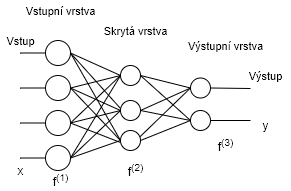
\includegraphics[width=0.6\linewidth]{obrazky/NNSchema.png}\\[1pt]  
    \caption{Schéma neuronové sítě}    
    \label{obrazekSchemaNeuronoveSite}
\end{figure*}

Úkolem neuronové sítě je aproximovat neznámou funkci $ y=f'(x)$
funkcí $ y=f(x;\theta )$, kde \emph{x} a \emph{y} značí vstup, 
respektive výstup.
K hodnotě $\theta$ dojde neuronová síť tak,
aby výsledný model nejlépe aproximoval původní funkci.
Samotná funkce \emph{f} se skládá z několika zřetězených funkcí 
$f(x)=f^{(3)}(f^{(2)}(f^{(1)}(x)))$,
kde $f^{(n)}$ označuje vrstvy sítě, 
jejichž vstupem je vektor z předchozí vrstvy 
a výstupem je opět vektor.
\cite{Goodfellow-et-al-2016}

\subsection*{Neurony}
Mnohem obvykleji jsou vrstvy reprezentovány množinou uzlů, 
které nazýváme neurony.
Vstupem každého neuronu je celý vektor předchozí vrstvy 
a výstupem je skalární hodnota, prvek výstupního vektoru jeho vrstvy.
Paralelním výpočtem všech neuronů vrstvy je získán její výsledek.
\cite{Goodfellow-et-al-2016}
\par

Každému vstupu neuronu je přiřazena váha, která jej buď posílí nebo utlumí.
Suma všech váhovaných vstupů poté prochází takzvanou aktivační funkcí,
která určuje jestli, a jak moc může signál pokračovat skrz síť.
Pokud signál projde, pak o neuronu můžeme říct, že byl aktivován.
\cite{Nicholson_NeuralNets}

\begin{figure*}[h]\centering
    \centering
    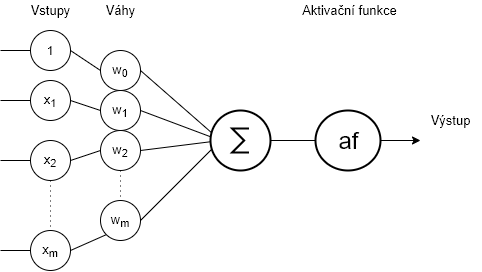
\includegraphics[width=0.6\linewidth]{obrazky/neuronSchema.png}\\[1pt]  
    \caption{Schéma neuronu}    
    \label{obrazekSchemaNeuronu}
\end{figure*}

\todo{TODO - Dopsat princip uceni NN}

\section{Rekurentní neuronové sítě}
Samotné neuronové sítě jsou pro některé typy problémů pořád příliš omezené.
Jejich vstupem je vektor pevně dané velikosti, 
výpočet probíhá v předem známém počtu kroků 
a na jeho konci je opět vektor pevné délky.
Taková omezení neberou v úvahu proudová data, 
tedy sekvence na sobě závislých vektorů.
Rekurentní sítě umožňují mít takovou sekvenci jako vstup, 
jako výstup, nebo jako obojí.
\cite{Karpathy_RNNs}.

\begin{figure*}[h]\centering
    \centering
    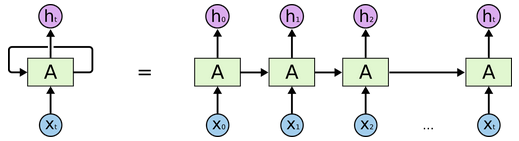
\includegraphics[width=0.6\linewidth]{obrazky/RNNSchema.png}\\[1pt]  
    \caption{Schéma rekurentní neuronové sítě\cite{colah_lstm}}    
    \label{obrazekSchemaRekurentniNeuronoveSite}
\end{figure*}

\section{LSTM}
\label{lstmTeorie}
Long Short-Term Network (dále jen LSTM), 
jsou speciálním druhem rekurentních neuronových sítí.
Jsou schopny se naučit i dlouhodobější závislosti v sekvencích dat.
S touto vlastností byly primárně navrženy.\cite{colah_lstm}
\par

Narozdíl od RNN mají LSTM čtyři vrstvy v jednom opakujícím se modulu.

% frameworky ... viz NOTES.md

\chapter{Návrh systému}
\label{navrhSystemu}
V této kapitole je představen návrh systému,
který umožní automatické generování harmonie na základě známé melodie.
Jak bylo napsáno, harmonie je souzvuk více zvuků najednou.
Aby systém dokázal generovat tóny, které spolu opravdu souzní,
musí obsahovat správně naučený model se správnými vstupy a výstupy.

\section{Vstup}
Vstupem celého systému je MIDI soubor, obsahující melodii,
pro kterou chceme vygenerovat harmonický doprovod.
Neuronové sítě si ale s takovými soubory neumí moc poradit,
a tak je soubor potřeba převést na vhodnější reprezentaci.
Podle \cite{google_git_polyphony} jsou touto reprezentací protocol buffers,
rychlejší a efektivnější datový formát než MIDI.
Protocol buffers je mechanismus firmy Google pro serializaci strukturovaných dat,
který je rozšiřitelný a nezávislý na jazyce a platformě, podobně jako například XML.
Veškeré protocol buffers zprávy jsou uložené v jednom .tfrecord souboru.
Definici zpráv určují takzvané .proto soubory.\cite{google_ProtocolBuffers}
V projektu Magenta se pro serializaci not používá jednotná definice zvaná NoteSequence.
\cite{google_musicColab}
\par

Pro trénování je vhodné samostatné serializované noty dále převést na SequenceExamples.
\cite{google_git_polyphony}
To je TensorFlow definice protocol bufferů určená k práci se sekvenčními daty.
Definice obsahuje dvě části -- context a feature\_lists.
Context obsahuje nesekvenční vlastnosti (features) jako například tempo a 
feature\_lists obsahuje sekvenční vlastnosti, jednotlivé noty.
Výhodou SequenceExamples je možnost distribuce trénování, 
kdy je možné rozdělit jeden .tfrecord soubor na více.
Další výhodou je znovupoužitelnost modelu, který SequenceExamples využívá.
Nevýhodou je velikost výsledných .tfrecord souborů s touto definicí oproti původním datům. 
\cite{britz_undocumentedFeatures}
Podle \cite{britz_undocumentedFeatures} může tento formát zvýšit velikost datové sady desetinásobně,
avšak při převedení všech MIDI souborů (viz kapitola \ref{hooktheoryDB}) 
je výsledná velikost $9.409e^3$krát vyšší (viz výpočet podle měření níže).

$$ tf / m = 94454904591B / 10038169B = 9.409575e^3$$

kde \emph{tf} je velikost všech výsledných .tfrecord souborů 
a \emph{m} je velikost všech vstupních MIDI souborů.

\section{Model}
Z modelů představených v kapitole \ref{prehledPristupus} byl vybrán 
Polyphony RNN z projektu Magenta.
V porovnání s ostatními přístupy je nejnovější a využívá framework TensorFlow
\cite{YinCheng_comparativeStudy,google_git_polyphony}.
Magenta poskytuje model\footnote{dostupný z \url{http://download.magenta.tensorflow.org/models/polyphony_rnn.mag}} 
již natrénovaný na chorálech, které složil Johann Sebastian Bach\footnote{
dostupné z \url{https://web.archive.org/web/20150503021418/http://www.jsbchorales.net/xml.shtml}, 
popřípadě z \url{https://github.com/cuthbertLab/music21/tree/master/music21/corpus/bach}}.
Kromě toho lze model natrénovat s pomocí vlastních dat,
kdy je také možné nastavit hyperparametry sítě jako například počet a velikost RNN vrstev.
\cite{google_git_polyphony}
\par

Primer modelu bude MIDI soubor se samotnou melodií, 
konvertovaný podle předchozí části na NoteSequence.
Úkolem systému je doplnění této melodie o složku harmonie, 
melodie proto bude použita jako součást výstupu.

\section{Výstup}
Výstupem samotného modelu je protocol buffer s definicí NoteSequence, 
stejně jako na vstupu.
Tato NoteSequence je interně převedena na výsledný MIDI soubor, 
který obsahuje původní melodii(primer), která je následována její harmonizovanou podobou.
\cite{google_git_polyphony}

\chapter{Trénování systému}
\label{trenovaniModelu}
% popis implementace
V této kapitole je představen postup zprovoznění systému a jeho trénování.
Vstupní data a postup jejich vytvoření je popsán v kapitole \ref{hooktheoryDB}.
Využitý systém je představen v části \ref{magenta} 
a podrobnější návrh potom v \ref{navrhSystemu}.
Postup harmonizace melodie modelem a provedené experimenty jsou popsány v kapitole následující.
\par

\section{Instalace}
Před začátkem trénování je nutné nainstalovat Magentu.
Jako testovací prostředí byl zvolen operační systém Ubuntu 20.04 LTS (Focal Fossa)
nainstalovaný na počítači s procesorem Intel Core i7-4720HQ s frekvencí 2.6GHz
a s 8Gb operační paměti. 
Pro instalaci knihovny na použitý operační systém je poskytnut instalační skript.

\begin{verbatim}
URL=https://raw.githubusercontent.com/tensorflow/ \
    magenta/master/magenta/tools/magenta-install.sh
curl $(URL) > /tmp/magenta-install.sh
bash /tmp/magenta-install.sh    
\end{verbatim}

Instalační skript nainstaluje Python distribuci Anaconda\footnote{\url{https://www.anaconda.com/}}
a s pomocí systému pro správu balíků \emph{conda} vytvoří nové virtuální prostředí \emph{magenta}.
Do tohoto prostředí dále nainstaluje potřebné balíky.
Mimo jiné například TensorFlow, magenta, scipy a numpy.
Pro prohlížení průběhu trénování je také nainstalován vizualizační nástroj TensorBoard.
Po dokončení instalace je potřeba restartovat okno s terminálem,
aby se načetly nové, změněné proměnné prostředí.
Nové, virtuální prostředí, které obsahuje korektní instalaci knihovny Magenta,
se aktivuje příkazem

\begin{verbatim}
source activate magenta
\end{verbatim}

Nyní jsou knihovna Magenta a všechny její závislosti 
připraveny k použití v Pythonu a v Jupyter sešitech.
Mimo to jsou Magenta skripty zavedeny v proměnné \emph{PATH}.
\cite{google_git_polyphony}
\par

\section{Příprava dat}
Dalším krokem je převedení sady trénovacích MIDI souborů na protocol buffer soubor
s definicí NoteSequence.
K tomuto účelu existuje skript \emph{convert\_dir\_to\_note\_sequences}, 
který sekvenčně načte složku obsahující MIDI (případně MusicXML, nebo ABC) soubory,
zkonvertuje je na NoteSequence a výsledek uloží do .tfrecord souboru.
Jeho chování lze ovlivnit argumenty.
Vstupní složka a výsledný soubor jsou jediné dva povinné parametry.
Parametry pro nastavení jsou \emph{input\_dir}, respektive \emph{output\_file}.
Pro rekurzivní procházení adresářů je nutno nastavit parametr \emph{recursive}.
\cite{google_git_polyphony}
Použití  pak vypadá následovně:

\begin{verbatim}
convert_dir_to_note_sequences \
    --input_dir=./midi \
    --output_file=./tmp/notesequences.tfrecord \
    --recursive
\end{verbatim} 

Konverze souborů ze složky \emph{./midi} netrvá dlouho
a výsledný soubor \emph{./tmp/notesequences.tfrecord}
má velikost $29.7$MB ($31 244 793$B)
\par

Nyní je nutné vytvořit SequenceExample soubory,
s jejichž pomocí bude model trénován a vyhodnocován.
Každá SequenceExample zpráva obsahuje sekvenci vstupů a
sekvenci příslušných označení, 
která reprezentuje polyfonní, harmonizovanou sekvenci.
Toho lze dosáhnout voláním příkazu \emph{polyphony\_rnn\_create\_dataset}.
Pomocí povinných parametrů \emph{input} a \emph{output\_dir} 
je nastaven vstupní soubor a složka pro uložení výsledků.
Parametrem \emph{eval\_ratio} se nastavuje, kolik procent dat 
bude použito jako datová sada určená k vyhodnocení modelu,
a kolik jako datová sada k trénování modelu.
\cite{google_git_polyphony}
Příkaz se správnými argumenty je

\begin{verbatim}
polyphony_rnn_create_dataset \
    --input=./tmp/notesequences.tfrecord \
    --output_dir=./tmp/polyphony_rnn/sequence_examples \
    --eval_ratio=0.10
\end{verbatim}

Generování trénovacích dat trvá zhruba čtyři až šest hodin.
Ve složce \emph{./tmp/polyphony\_rnn/sequence\_examples} budou po dokončení
dva soubory. 
Jeden s trénovacími daty, \emph{training\_poly\_tracks.tfrecord},
který obsahuje 90\% dat,
a druhý, \emph{eval\_poly\_tracks.tfrecord} s daty pro vyhodnocení modelu.
Tento obsahuje zbývajících 10\% dat.
Velikost obou souborů dohromady je $8.39GB + 79.5GB = 87.9GB$ ($94 454 904 591$B).
\par

\section{Trénování}
Nyní je vše připraveno k trénování modelu.
Příslušný příkaz lze ovlivnit několika parametry.
S pomocí \emph{run\_dir} je určena cesta k adresáři,
který je určen k ukládání průběžných výsledků trénování (checkpoints), 
a k ukládání souhrných dat pro TensorBoard.
Uvnitř tohoto adresáře jsou dva podadresáře,
do nichž jsou uložena zvlášť data z trénování a z vyhodnocení modelu.
Souhrnná data se ukládají každý desátý krok.
Pro změnu kroku existuje parametr \emph{summary\_frequency}.
Průběžné výsledky trénování nejsou ukládány všechny, 
nýbrž pouze posledních deset.
Toto číslo lze opět změnit parametrem \emph{num\_checkpoints}.
Při jeho nastavení na nulu jsou uloženy všechny a žádný se nemaže.
Cesta k trénovacím, případně vyhodnocovacím datům, 
je dána parametrem \emph{sequence\_example\_file}.
Nepovinný parametr \emph{num\_training\_steps} určuje,
kolik trénovacích cyklů model prodělá, než se trénování ukončí.
Pokud tento není zadán, trénování pokračuje nepřetržitě, 
dokud není manuálně ukončeno.
Vyhodnocení modelu se aktivuje parametrem \emph{eval}.
Při jeho nastavení nejsou aktualizovány váhy modelu.
Posledním důležitým, ale nepovinným parametrem je \emph{hparams}.
Tímto lze změnit základní nastavení hyperparametrů modelu.
Jedná se o seznam dvojic klíč-hodnota oddělených čárkami,
kde klíč je jméno měněného hyperparametru a hodnota je nová hodnota, 
na kterou bude tento změněn.
Takto zadané hyperparametry jsou sloučeny s původními.
Jména hyperparametrů jsou batch\_size a rnn\_layer\_sizes.
Prvním se nastavuje počet SequenceExample zpráv, trénovacích dat,
které jsou použity na jeden průchod sítí, po kterém se provede aktualizace vah.
Základní nastavení je 128 zpráv.
Druhým se nastavuje velikost sítě.
Jedná se o pole čísel, kde každý prvek pole značí jednu RNN vrstvu,
a hodnota prvku udává počet neuronů dané vrstvy.
Výchozí hodnoty vytvoří síť se třemi vrstvami, 
každá o 256 neuronech. 
\cite{google_git_polyphony}
Pro zkrácení doby učení a snížení paměťové náročnosti budou použity jiné, nižší hyperparametry.
Příkaz pro trénování Polyphony RNN na vlastní datové sadě tak bude vypadat následovně:

\begin{verbatim}
polyphony_rnn_train \
    --run_dir=./tmp/polyphony_rnn/logdir/run1 \
    --sequence_example_file=./tmp/polyphony_rnn/sequence_examples/training_poly_tracks.tfrecord \
    --hparams="batch_size=64,rnn_layer_sizes=[64,64]" \
    --num_training_steps=20000
\end{verbatim}

S tímto nastavení trvá trénování na testovacím počítači přibližně 25 hodin.
Skript průběžně zapisuje statistiky o právě probíhajícím cyklu, 
včetně průměrného počtu cyklů za vteřinu.
Pomocí této hodnoty lze odhadnout dobu trvání trénování při jiných hyperparametrech.

        \todo{Dopsat podle odhadnuté hodnoty}

\par

Volitelně je možné paralelně spustit stejný skript s přidaným parametrem \emph{eval},
což spustí vyhodnocovací úlohu.
V tomto případě bude po každém trénovacím cyklu proveden vyhodnocovací cyklus.
Vyhodnocení se provede vždy po dokončení cyklu učení, 
a není tedy možné tento příkaz spustit po dokončení trénování.
\cite{google_git_polyphony}


\begin{verbatim}
polyphony_rnn_train \
    --run_dir=./tmp/polyphony_rnn/logdir/run1 \
    --sequence_example_file=./tmp/polyphony_rnn/sequence_examples/training_poly_tracks.tfrecord \
    --hparams="batch_size=64,rnn_layer_sizes=[64,64]" \
    --num_training_steps=20000 \
    --eval
\end{verbatim}  
\par

Průběh trénovacího a vyhodnocovacího procesu lze sledovat na adrese
\url{http://localhost:6006} po spuštění TensorBoard nástroje příkazem

\begin{verbatim}
tensorboard --logdir=./tmp/polyphony_rnn/logdir   
\end{verbatim}
\par

Po dokončení učení modelu je možné s ním experimentovat, 
a nechat jej harmonizovat melodie uložené v MIDI souborech.
Případně je možné používat model, který nedokončil všechny cykly určené v parametrech.
V tom případě se použijí váhy z posledního dokončeného cyklu.
\par
Naučený model ve formě posledních $n$ checkpointů lze transformovat
na více kompaktní, zabalený soubor.
Ten, kromě posledních checkpointů, obsahuje také graf a některá metadata modelu.
Příkaz \emph{polyphony\_rnn\_generate} s příznakem \emph{save\_generator\_bundle}
načte model ze složky uvedené v parametru \emph{run\_dir}.
Pro správnou funkci je nutné dodat stejný popis hyperparametrů v parametru \emph{hparams}, 
jaký byl použit při trénování.
Cesta k výslednému .mag souboru je určena v \emph{bundle\_file}.
Jedná se opět o zabalený protocol buffer, nyní však s definicí GeneratorBundle.
Zabalení modelu do jednoho souboru je vhodné při sdílení předtrénovaného modelu.
\cite{google_git_polyphony}


\begin{verbatim}
polyphony_rnn_generate \
    --run_dir=./tmp/polyphony_rnn/logdir/run1 \
    --hparams="batch_size=64,rnn_layer_sizes=[64,64]" \
    --bundle_file=./tmp/polyphony_rnn.mag \
    --save_generator_bundle
\end{verbatim}

\section{Použití modelu}
Generovat polyfonní a harmonizované skladby s použitým modelem
lze téměř od samého začátku.
Je ale vhodné jej nechat trénovat dostatečně dlouho.
Kromě toho lze použít také model zabalený v .mag souboru.
Chování generátoru upravuje několik parametrů.
Výběr modelu specifikují parametry \emph{run\_dir} a \emph{bundle\_file},
kdy první určuje cestu ke složce s trénovaným modelem (přesněji s uloženými checkpointy)
a druhý určuje cestu k .mag souboru s již natrénovaným modelem.
Při zadání obou má prioritu druhý popisovaný parametr.
Při použití parametru \emph{run\_dir} je nutné uvést
také parametr \emph{hparams} tak, jak byl použit při trénování 
(některé z uvedených hyperparametrů budou ignorovány, například batch\_size).
Složku pro uložení vygenerovaných MIDI souborů vymezuje parametr \emph{output\_dir}.
Počet nových souborů pak parametr \emph{num\_outputs}.
Každý generovaný soubor je rozdílný, liší se provedením harmonizace.
Je vhodné výsledky poslechnout a zjistit jejich kvalitu.
\par

Délka výsledné skladby je dána parametrem \emph{num\_steps} 
Jednotka délky kroku je v tomto případě šestnáctinová nota,
jinými slovy -- do vygenerované melodie se vleze právě \emph{num\_steps} šestnáctinových not.
Délka jednoho taktu je šestnáct kroků.
Problém tohoto modelu je, že do generované skladby nejdříve vloží melodii samotnou, 
jako primer popsaný v kapitole \ref{navrhSystemu}.
Je tedy nutné délku původní melodie násobit dvěma,
aby se do výsledného souboru dostala jak původní melodie,
tak její rozšířená část.
\cite{google_git_polyphony}

\par

Základ generátoru (primer ) lze specifikovat třemi způsoby.
Jelikož je model původně určený pro generování polyfonních skladeb,
je možné začít pouze jedním akordem.
Ten se vkládá parametrem \emph{primer\_pitches},
který obsahuje řetězec reprezentující Python pole.
Jednotlivé prvky tohoto pole jsou MIDI výšky tónů,
z nichž je tento akord složen.
Například celý parametr určující akord C dur vypadá následovně:

\begin{verbatim}
--primer_pitches="[67, 64, 60]"
\end{verbatim}

Ve vygenerované skladbě trvá základ, 
vložený tímto způsobem, první dobu (délka čtvrťové noty).
\par

Další možností je vložení počáteční melodie.
Ta je vložena ve formě Python pole, stejně jako v předchozím případě.
Noty ve formě MIDI výšek jsou doplněny o dvě řídící hodnoty.
Žádnou událost značí číslo $-2$ a 
deaktivace znějící noty (note-off) je reprezentována číslem $-1$.
Parametr pro tuto možnost je \emph{primer\_melody}.

\begin{verbatim}
--primer_melody="[60, -2, 60, -2, 67, -2, 67, -2 ]"  
\end{verbatim}

Poslední možností je načtení základní stopy z MIDI souboru,
jehož cesta je v parametru \emph{primer\_midi}.
\begin{verbatim}
--primer_midi=./primer.mid 
\end{verbatim}

Při použítí více než jednoho parametru pro vložení základu
mají parametry následující prioritu:
\begin{enumerate}
    \item primer\_pitches
    \item primer\_melody
    \item primer\_midi
\end{enumerate}
\par

Další parametry upravují použití základu generátorem.
Pokud je argument \emph{condition\_on\_primer} nastaven na true, 
pak je primer načten modelem ještě před začátkem generování nové sekvence.
Tento argument se používá dohromady s \emph{primer\_pitches} 
ke stanovení tóniny generované stopy jejím akordem.
Nastavením parametru \emph{inject_primer_during_generation} na true
bude poskytnutý základ použit jako součást generované skladby.
Toto chování se hodí právě pokud je úkolem harmonizace existující melodie.
V takovém případě by se neměl používat předchozí parametr \emph{condition\_on\_primer},
protože model nejdříve uvidí monofonní melodii 
a má generovat polyfonní.
\cite{google_git_polyphony}

% experiment s harmonizací melodie s akordama se zaplým condition
\par
Posledním pro experimenty zajímavým parametrem je \emph{temperature},
který ovlivňuje náhodnost generovaných stop.
Číslo větší než jedna znamená více náhodný výsledek,
naopak číslo menší než jedna vede k menší náhodnosti.
Výchozí hodnota je pochopitelně $1.0$.
\par

Celý příkaz pro vygenerování harmonie k melodii
uložené v MIDI souboru vypadá následovně:

\begin{verbatim}
polyphony_rnn_generate \
    --bundle_file=./tmp/polyphony_rnn.mag \
    --output_dir=./generated \
    --num_outputs=10 \
    --num_steps=268 \
    --primer_midi=./melody.mid \
    --condition_on_primer=false \
    --inject_primer_during_generation=true    
\end{verbatim}

\chapter{Experimenty}
% experimentování s implementovaným systémem
% představení výsledků
Tato kapitola popisuje možnosti natrénovaného modelu 
a jsou představeny provedené experimenty.
Model jako takový je popsán v kapitolách \ref{magenta} a \ref{navrhSystemu},
postup jeho zprovoznění, trénování a použití pak v kapitole \ref{trenovaniModelu}.
Použitá trénovací sada je popsána v kapitole \ref{hooktheoryDB}.
Model, na kterém byly experimenty prováděny, 
byl natrénován s hyperparametry, které byly představeny v minulé kapitole.
Tedy:
\begin{itemize}
    \item velikost dávky = 64
    \item počet RNN vrstev = 2
    \item neuronů v každé vrstvě = 64
    \item trénovacích cyklů = 20 000
\end{itemize}
\par
Parametry použité při generování, pokud není stanoveno jinak, jsou:
\begin{itemize}
    \item condition_on_primer=false
    \item inject_primer_during_generation=true
    \item bundle_file=./mnt/d/tmp/polyphony_rnn.mag
    \item num_outputs=10 
    \item temperature=1.0
\end{itemize}

\section{Harmonizace krátké melodie}
Prvním experimentem nechť je harmonizace skladby o pouhých dvou taktech,
která se nacházela v trénovací datové sadě 
(viz noty na obrázku \ref{obrazekNotyKratkeZname},
případně pianoroll MIDI souboru na obrázku \ref{obrazekPianoRollKratkeZname}).
Modelu známá melodie by měla vyústit ve harmonii velmi podobnou té původní.
Naproti tomu je melodie velmi krátká.
Pro extrakci samotné melodie z MIDI souboru obsahující tuto skladbu 
byl vytvořen krátký Python skript \emph{harmonizer/melodyFromMidi.py}, 
který jako první parametr přijímá cestu k tomuto souboru.

\begin{figure*}[h]\centering
    \centering
    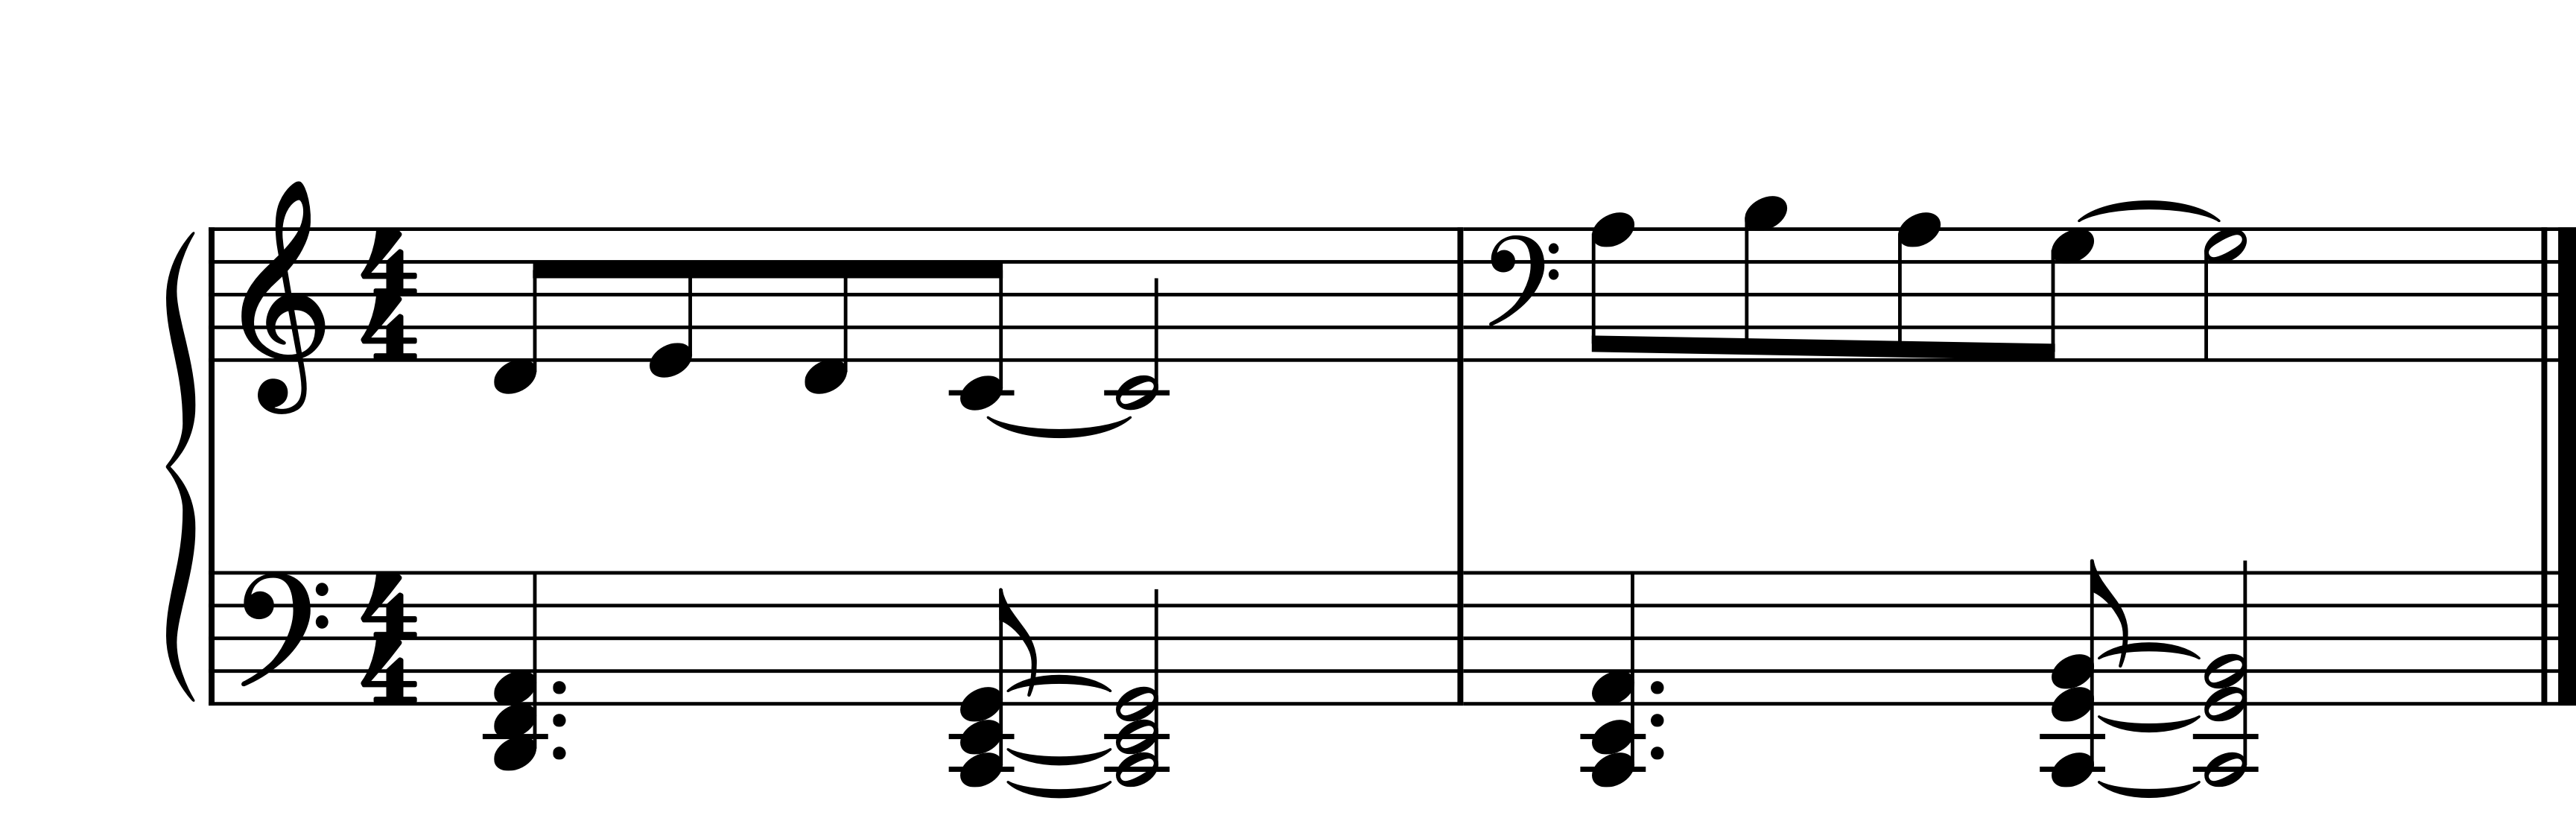
\includegraphics[width=0.8\linewidth]{obrazky/KratkaSkladbaKHarmonizaciNoty.png}\\[1pt]  
    \caption{Notový zápis použité skladby. Horní osnova je melodie, spodní harmonie.}    
    \label{obrazekNotyKratkeZname}
\end{figure*}
\begin{figure*}[h]\centering
    \centering
    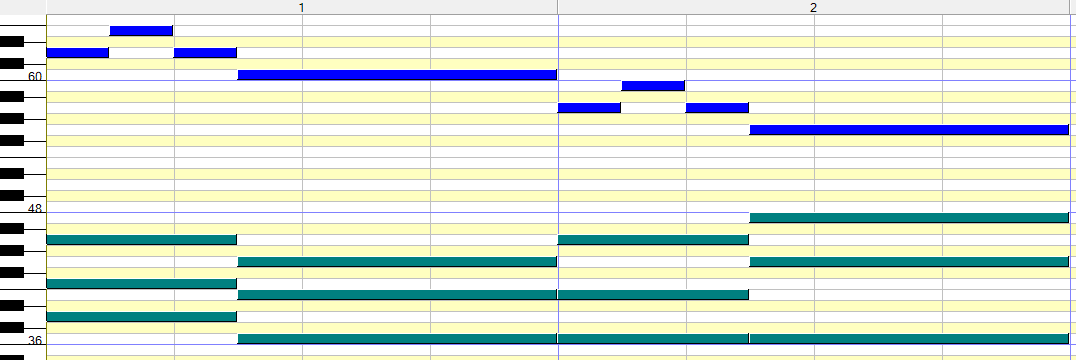
\includegraphics[width=0.8\linewidth]{obrazky/KratkaSkladbaKHarmonizaciPianoRoll.png}\\[1pt]  
    \caption{Pianoroll použité skladby. Modré obdélníky jsou melodie, zelené harmonie.
    Vertikální osa jsou MIDI výšky tónů, zatímco horizontální je čas. 
    Čísla nahoře značí první a druhý takt skladby.}    
    \label{obrazekPianoRollKratkeZname}
\end{figure*}

Harmonizace byla provedena čtyřikrát 
s různou hodnotou parametru temperature.
Nejprve byly generovány soubory s výchozí hodnotou ($1.0$),
poté s nižší ($0.7$) a nakonec dvakrát s vyššími hodnotami ($1.3$, respektive $2.0$).
Při každém běhu bylo vytvořeno 10 souborů,
které byly ručně analyzovány a poslechnuty.
\par

Skladby generované s nízkou hodnotou temperature vykazovaly,
jak předpovídala dokumentace, vyšší náhodnost vytvořených tónů.
Model většinou používá mnoho krátkých akordů, 
ne vždy ale začínají ve správný čas, akordy nedoplňují melodii 
a celkově je poslech těchto skladeb ne příliš příjemný.
Existují ovšem výjimky, viz notový zápis na obrázku 
\ref{obrazekKratkaSkladbaHarmonizovanaLowNoty},
kde doplněné noty původní melodii rozvádí přechody mezi jednotlivými akordy.

\begin{figure*}[h]\centering
    \centering
    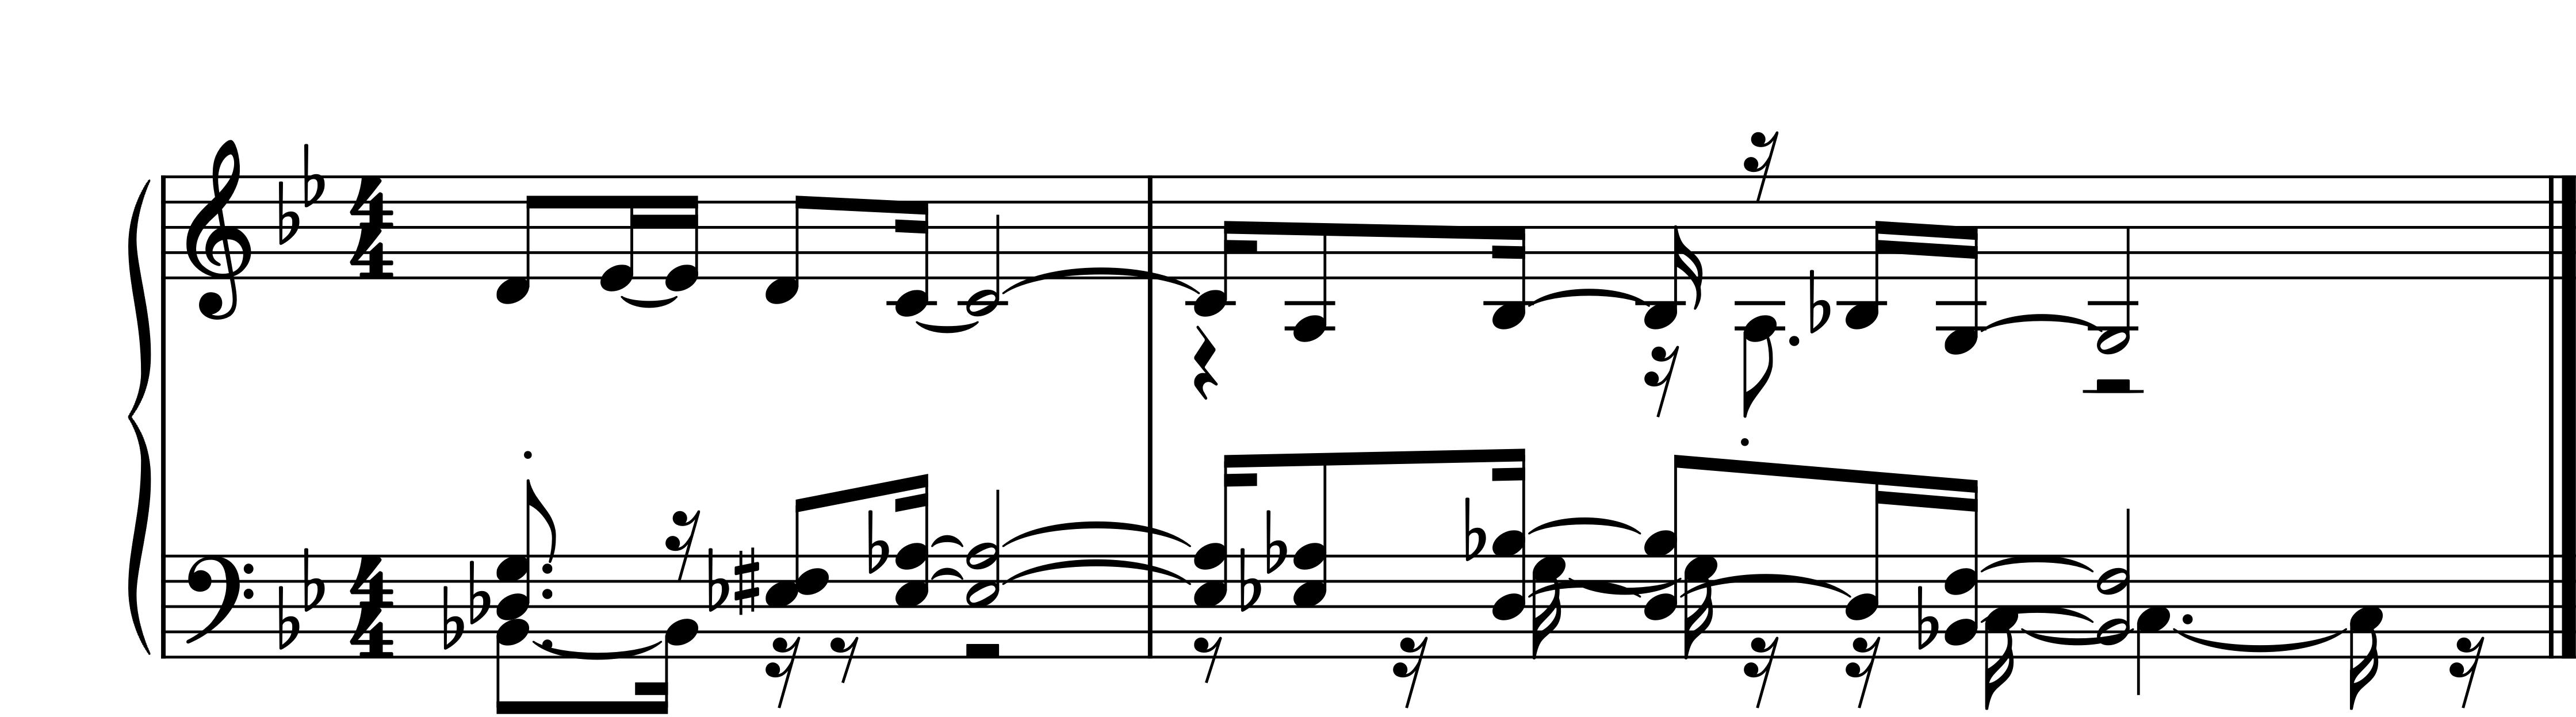
\includegraphics[width=0.8\linewidth]{obrazky/KratkaSkladbaHarmonizovanaLowNoty.png}\\[1pt]  
    \caption{Notový zápis vygenerované skladby}    
    \label{obrazekKratkaSkladbaHarmonizovanaLowNoty}
\end{figure*}
\par

Harmonizace prováděná s výchozí hodnotou temperature 
byly obecně příjemnější k poslechu než předchozí přístup.
Akordy začínaly zároveň s tóny původní melodie a byly delší.
U některých výsledků se však vyskytoval jistý nešvar, 
totiž tóny akordů trvající velmi dlouho, někdy i déle než jeden takt.
Poslech tak ovlivňuje i nastavený hudební nástroj při syntéze MIDI souboru,
neboť některé se rozezní pouze na začátku MIDI události, ale brzy dozní
a po zbytek události je tón neslyšitelný.
Pro správný poslech je tak nutné nastavit MIDI nástroj, který zní celou dobu
(například \emph{16-Varhany}, nebo \emph{40-Housle}).
Toto chování lze připsat použité datové sadě,
kdy se na serveru www.hooktheory.com vkládají většinou pouze harmonizační funkce akordů,
které trvají i více taktů a nemění se tak často.
\par
V některých případech také model těsně před koncem skladby vygeneruje změnu akordu,
který má tendenci v melodii pokračovat (viz obrázek \ref{obrazekKratkaSkladbaHarmonizovanaDefNoty}).

\begin{figure*}[h]\centering
    \centering
    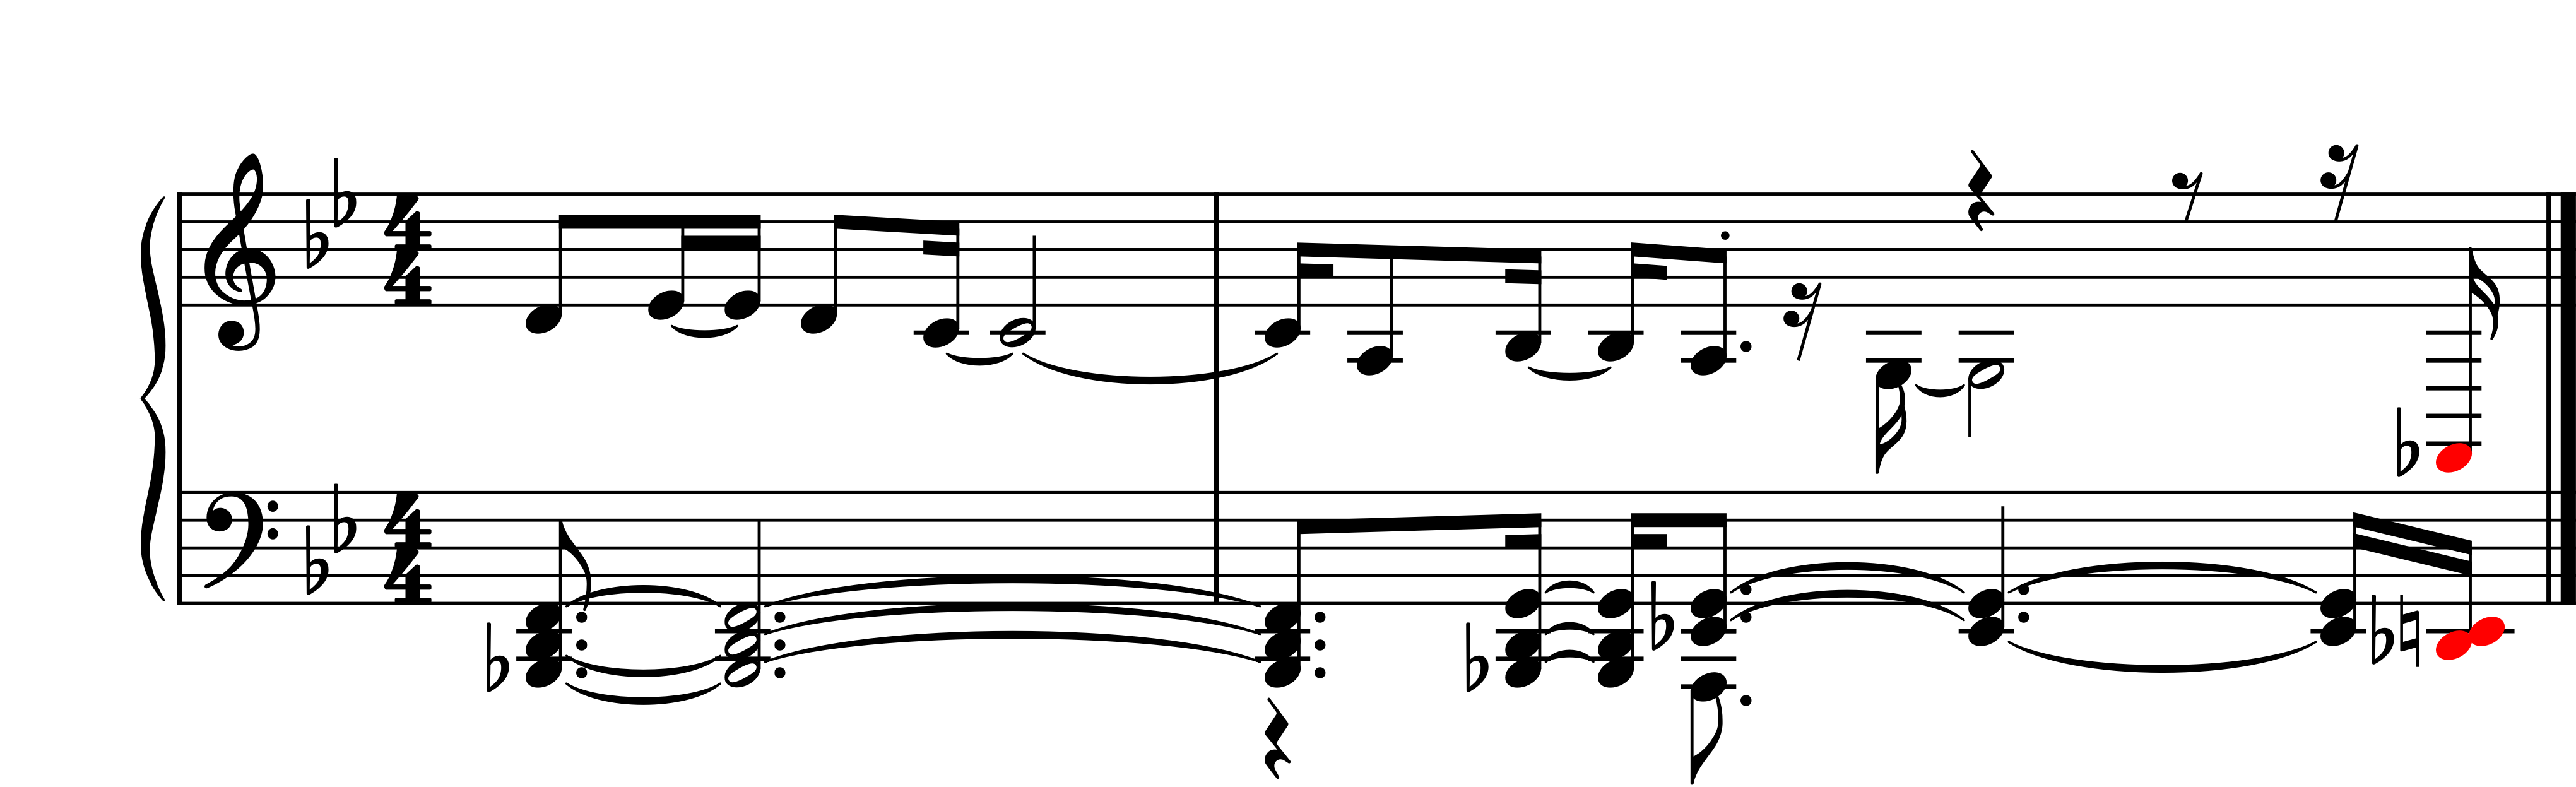
\includegraphics[width=0.8\linewidth]{obrazky/KratkaSkladbaHarmonizovanaDefNoty-1.png}\\[1pt]  
    \caption{Notový zápis vygenerované skladby s výchozím parametrem temperature. 
    Červené noty znázorňují náhlou změnu na konci skladby.}    
    \label{obrazekKratkaSkladbaHarmonizovanaDefNoty}
\end{figure*}
\par

Dva běhy harmonizace s parametrem temperature vyšším než původním
dále prodlužovaly použité akordy.
Harmonie byla také více předvídatelná a tolik se neměnily použité akordy.
Pokusy o pokračování skladby se objevovaly spíše zřídka.
Zdařilá harmonizace s tímto nastavením je na obrázku 
\ref{obrazekKratkaSkladbaHarmonizovanaHighNoty}.

\begin{figure*}[h]\centering
    \centering
    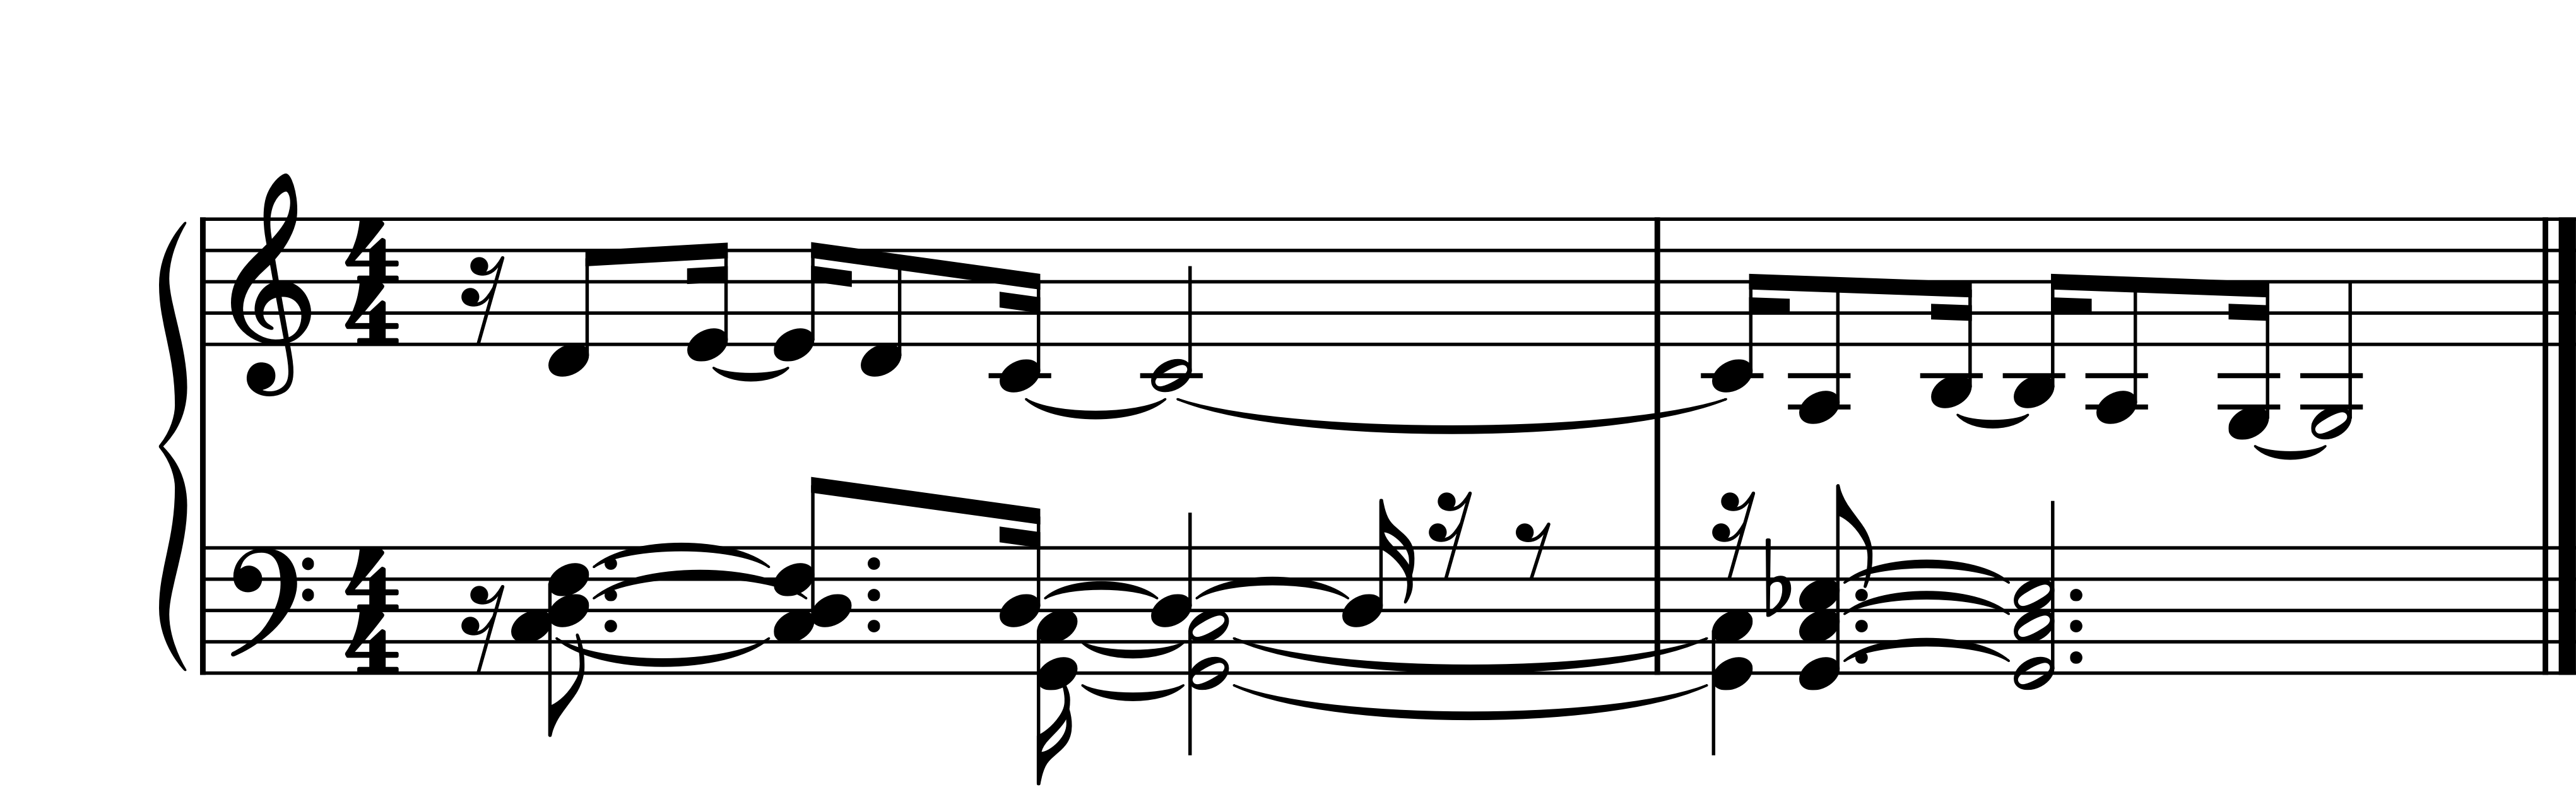
\includegraphics[width=0.8\linewidth]{obrazky/KratkaSkladbaHarmonizovanaHighNoty-1.png}\\[1pt]  
    \caption{Notový zápis vygenerované skladby s vyšším parametrem temperature. 
    Tóny harmonie trvají několik dob.}    
    \label{obrazekKratkaSkladbaHarmonizovanaHighNoty}
\end{figure*}
\par

\chapter{Diskuse}
% diskuse výsledků
% jak je použít
% srovnání s cizími pracemi a papery

\chapter{Závěr}
\label{zaver}
% shrnutí práce
% možný budoucí vývoj práce
% celkový přínos
Cílem této práce bylo seznámit se s harmonizací známé melodie a 
s možností automatizace této činnosti za pomoci neuronových sítí.
Následně navrhnout systém, který bude automatickou harmonizaci umožňovat.
\par

Základům hudby byla věnována první kapitola, 
další se popisovala různé přístupy k automatické harmonizaci. 
Některé poznatky z těchto prací byly vybrány a použity v návrhu v následující kapitole.
Na základě tohoto návrhu bude poté, ve výsledné diplomové práci, 
implementován systém a jeho neuronová síť s využitím frameworku PyTorch.
Toto řešení bude, na základě testovacích dat, vyhodnoceno.
V závěru budou diskutovány výsledky a možné pokračování této práce.
